%  article.tex (Version 3.3, released 19 January 2008)
%  Article to demonstrate format for SPIE Proceedings
%  Special instructions are included in this file after the
%  symbol %>>>>
%  Numerous commands are added out, but included to show how
%  to effect various options, e.g., to print page numbers, etc.
%  This LaTeX source file is composed for LaTeX2e.

%  The following commands have been added in the SPIE class
%  file (spie.cls) and will not be understood in other classes:
%  \supit{}, \authorinfo{}, \skiplinehalf, \keywords{}
%  The bibliography style file is called spiebib.bst,
%  which replaces the standard style unstr.bst.

%\documentclass[a4paper]{spie}
\documentclass[]{spie}  %>>> use for US letter paper
%%\documentclass[a4paper]{spie}  %>>> use this instead for A4 paper
%%\documentclass[nocompress]{spie}  %>>> to avoid compression of citations
%% \addtolength{\voffset}{9mm}   %>>> moves text field down
%% \renewcommand{\baselinestretch}{1.65}   %>>> 1.65 for double spacing, 1.25 for 1.5 spacing
%  The following command loads a graphics package to include images
%  in the document. It may be necessary to specify a DVI driver option,
%  e.g., [dvips], but that may be inappropriate for some LaTeX
%  installations.
\usepackage[]{graphicx}
\usepackage{color}
\usepackage{cancel}
\usepackage{amsmath}
\usepackage{amsfonts}
\usepackage{mathtools}
\usepackage{verbatim}
\usepackage{titlesec}
\definecolor{linkcolor}{cmyk}{1, 0.65, 0, 0.3}			% PANTONE 288 CVU
\definecolor{citecolor}{cmyk}{0.79, 0, 0.87, 0.56}		% PANTONE 357 CVU
%\definecolor{citecolor}{cmyk}{1, 0, 0.47, 0.3}			% PANTONE 328
\def\red{\textcolor{red}}
\def\blue{\textcolor{blue}}
\usepackage[
	colorlinks,
	linkcolor=linkcolor,
	urlcolor=linkcolor,
	citecolor=linkcolor,
	pdftex,
	pdfstartview=FitH,
]{hyperref}

\titleformat{\section}{\normalfont\fontsize{11.5pt}{1em}\bfseries}{SUPPLEMENTARY NOTE \thesection: }{0em}{}
\titleformat{\subsection}{\normalfont\fontsize{11pt}{0.75em}\bfseries}{SUPPLEMENTARY NOTE \thesubsection: }{0em}{}
\titleformat{\subsubsection}{\normalfont\fontsize{11pt}{0.75em}\bfseries}{SUPPLEMENTARY NOTE \thesubsubsection: }{0em}{}

% jump to the top of a figure, not the caption
\usepackage[all]{hypcap}

% so that footnotes in tables work
\usepackage{footnote}

% so that we can omit the 'Table 1:' for the overview
\usepackage{caption}

% should be called Supplementary Figure
\renewcommand{\figurename}{Supplementary Figure}

% for the source code
\usepackage{listings}

\usepackage{helvet}
\renewcommand{\rmdefault}{\sfdefault}
\renewcommand{\baselinestretch}{1.05}

%\usepackage{sectsty}Bayesian-based single-view and multi-view deconvolution
%\allsectionsfont{\sffamily}

\captionsetup[table]{labelformat=empty}

\newcommand\smallurl[1]{{\small{\url{#1}}}}
\newcommand\tablespace{\vspace{2.5mm}}
\newcommand\fig{supplementary figure }
\newcommand\Fig{Supplementary figure }


\title{BigStitcher: Efficient alignment of large multi-tile and multi-view image datasets}

%>>>> The author is responsible for formatting the
%  author list and their institutions.  Use  \skiplinehalf
%  to separate author list from addresses and between each address.
%  The correspondence between each author and his/her address
%  can be indicated with a superscript in italics,
%  which is easily obtained with \supit{}.

\author{David H{\"o}rl, Fabio Rojas Rusak, Stephan Preibisch
%\skiplinehalf
%\small{
%\supit{1}Max Planck Institute of Molecular Cell Biology and Genetics, Pfotenhauerstrasse 108, Dresden, Germany \\
%\supit{2}HHMI Janelia Farm Research Campus, 19700 Helix Drive, Ashburn, VA 20147, USA \\
%\supit{3}Albert Einstein College of Medicine, 1300 Morris Park Avenue, Bronx, NY 10461, USA
%}
}

%>>>> Further information about the authors, other than their
%  institution and addresses, should be included as a footnote,
%  which is facilitated by the \authorinfo{} command.

%\authorinfo{Further author information: (Send correspondence to A.A.A.)\\A.A.A.: E-mail: aaa@tbk2.edu, Telephone: 1 505 123 1234\\  B.B.A.: E-mail: bba@cmp.com, Telephone: +33 (0)1 98 76 54 32}
%%>>>> when using amstex, you need to use @@ instead of @


%%%%%%%%%%%%%%%%%%%%%%%%%%%%%%%%%%%%%%%%%%%%%%%%%%%%%%%%%%%%%
%>>>> uncomment following for page numbers
\pagestyle{plain}
%>>>> uncomment following to start page numbering at 301
%\setcounter{page}{1}

% underset argument for (arg)max/min
\DeclareMathOperator*{\argmax}{arg\,max}
\DeclareMathOperator*{\argmin}{arg\,min}
%\DeclareMathOperator*{\max}{max}
%\DeclareMathOperator*{\min}{min}
%\DeclareMathOperator{\deg}{deg}

\begin{document}

\maketitle

%\pagestyle{headings}
\setcounter{page}{1}
\pagenumbering{roman}
\pagenumbering{arabic}


\hspace{20mm}

\begin{table}[h!]
\center
{
\fontsize{12pt}{11pt}\selectfont
\center
\begin{tabular}{lp{11cm}}
\textbf{\textcolor{red}{Supplementary File}} & \textbf{\textcolor{red}{Title}}\\ \\
\hline
\\
\textbf{Supplementary Figure \ref{fig:sup-fig-rf}} & Fluorescence preservation in cleared samples\tablespace \\
\textbf{Supplementary Figure \ref{fig:sup-fig-illu-select}} & Automatic illumination selection \tablespace \\
\textbf{Supplementary Figure \ref{fig:sup-fig-manual-align1}} &  Manual alignment \tablespace \\
\textbf{Supplementary Figure \ref{fig:sup-fig-flatfield}} & Flat-field correction \tablespace \\
\textbf{Supplementary Figure \ref{fig:sup-fig-globalopt}} & Global optimization \tablespace \\
\textbf{Supplementary Figure \ref{fig:sup-fig-stitching}} & Pairwise registration by phase correlation \tablespace \\
\textbf{Supplementary Figure \ref{fig:sup-fig-downsampling}} & Downsampling with different SNR \tablespace \\
\textbf{Supplementary Figure \ref{fig:sup-fig-downsampling-statistics-0}} & Downsampling error statistics 1 \tablespace \\
\textbf{Supplementary Figure \ref{fig:sup-fig-downsampling-statistics-1}} & Downsampling error statistics 2 \tablespace \\
\textbf{Supplementary Figure \ref{fig:sup-fig-downsampling-statistics-2}} & Downsampling error statistics 3 \tablespace \\
\textbf{Supplementary Figure \ref{fig:sup-fig-link-explorer}} & Interactive inspection and curation of pairwise links \tablespace \\
\textbf{Supplementary Figure \ref{fig:sup-fig-icp}} & Affine refinement via ICP \tablespace \\
\textbf{Supplementary Figure \ref{fig:sup-fig-boundingbox}} & Bounding Box definition \tablespace \\
\textbf{Supplementary Figure \ref{fig:sup-fig-fusion}} & Virtual fusion of large image \tablespace \\
\textbf{Supplementary Figure \ref{fig:sup-fig-interest-point}} & Interest point visualization \tablespace \\
\textbf{Supplementary Figure \ref{fig:sup-fig-manual-align2}} & Manual Transformation of multi-view datasets \tablespace \\
\textbf{Supplementary Figure \ref{fig:sup-fig-expansion-microscopy}} & Expansion Microscopy Stitching \tablespace \\
\textbf{Supplementary Note \ref{sec:sup-note1}-\ref{sec:fusion}} & Supplementary methods \tablespace \\
\textbf{Supplementary Note \ref{sec:documentation}} & BigStitcher User Guide \tablespace \\
\textbf{Supplementary Note \ref{sec:currentcode}} & Links to the current source codes \tablespace \\

\end{tabular}}
\caption{\emph{Note: Supplementary Videos 1--5 are available for download on the journal homepage.}}
\end{table}

\pagebreak

\titleformat{\section}{\centering\normalfont\fontsize{13.5pt}{1em}\bfseries}{SUPPLEMENTARY NOTE \thesection: }{0em}{}
\section*{SUPPLEMENTARY FIGURES}
\titleformat{\section}{\normalfont\fontsize{11.5pt}{1em}\bfseries}{SUPPLEMENTARY NOTE \thesection: }{0em}{}


\subsection*{SUPPLEMENTARY FIGURE 1: Fluorescence preservation in cleared samples}
\vspace{1mm}
\begin{figure*}[ht!]
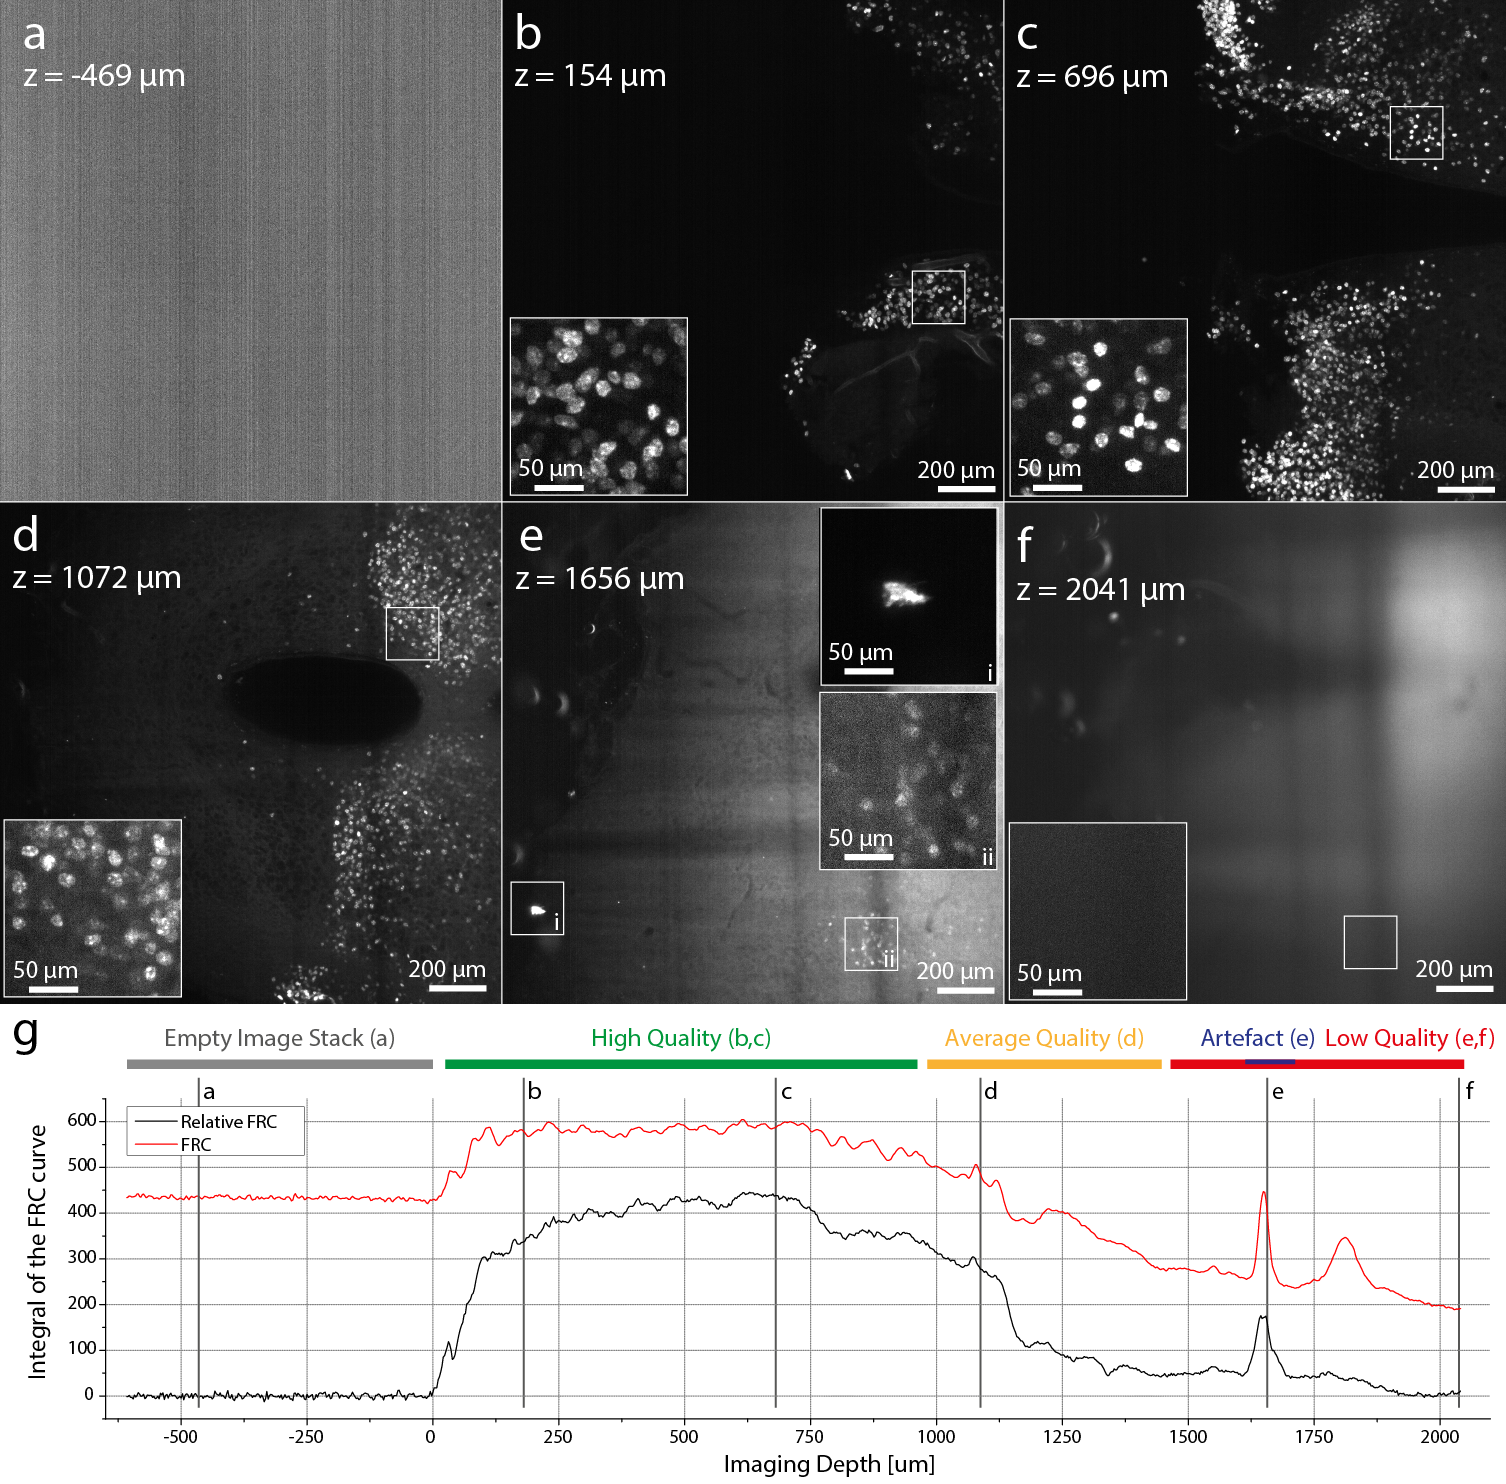
\includegraphics[width=\textwidth]{fig-rf.png}
\vspace{-2.0mm}
\caption{\hspace{-0.5mm} \emph{Fluorescence preservation and image analysis in cleared samples.} \textbf{(a)-(d)} Optical sections through an adult mouse hypothalamus in a CLARITY-cleared adult mouse brain expressing H2B-GFP in all bsx neurons. Fluorescence is preserved throughout the clearing procedure and can be used in advanced image analyses. The examples shows nuclear segmentation of pixel-wise classification using a Random Forest \cite{arganda2017trainable} model. Classification results (probability maps) are overlaid in blue onto the grayscale raw intensities.
}
\label{fig:sup-fig-rf}
\end{figure*}

\subsection*{SUPPLEMENTARY FIGURE 2: Automatic illumination selection}
\vspace{1mm}
\begin{figure*}[h!]
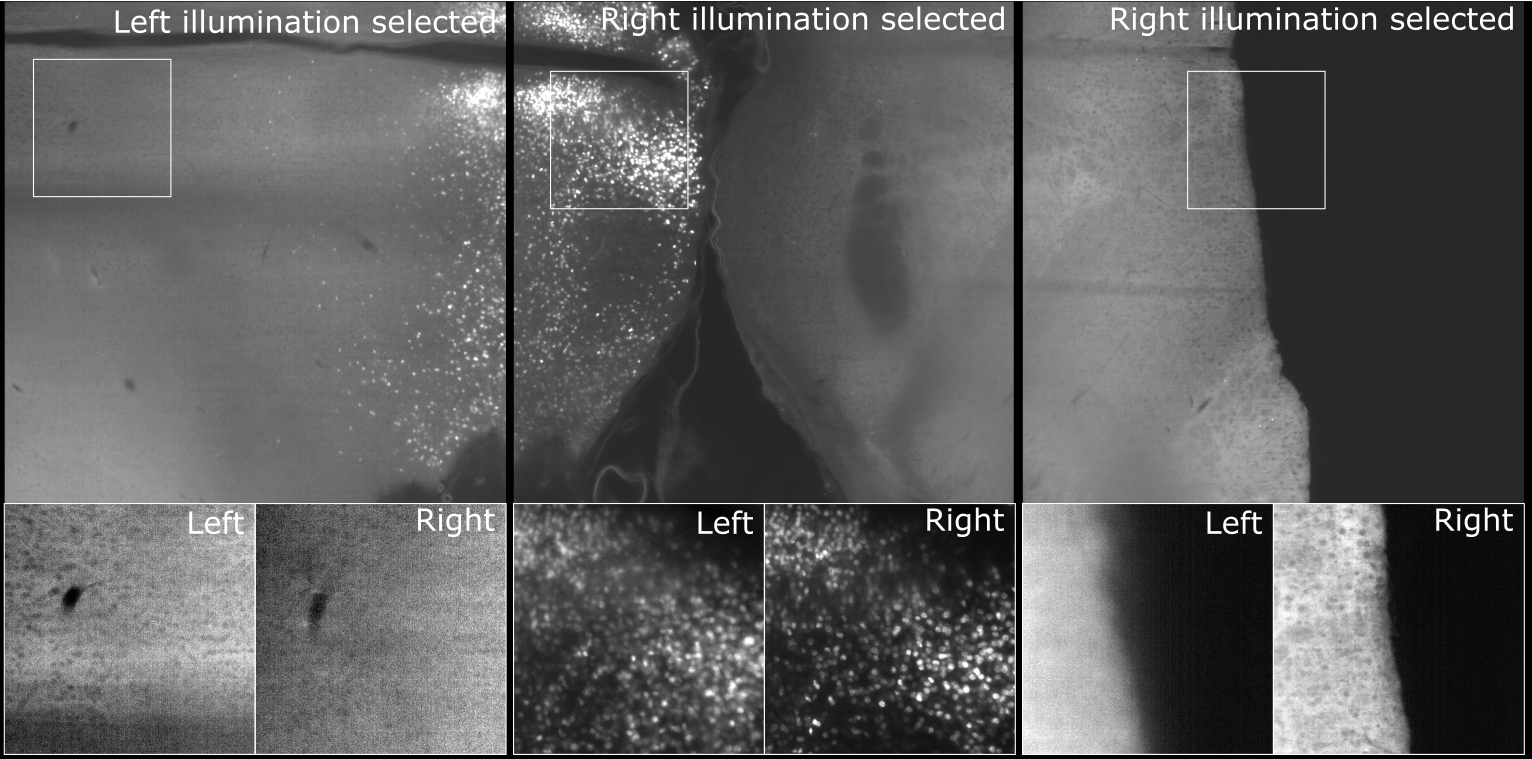
\includegraphics[width=\textwidth]{Illu_Select.png}
\vspace{-2.0mm}
\caption{\hspace{-0.5mm} \emph{Automatic illumination selection.} Best illumination for three consecutive tiles was selected based on brightest view for each tile. Close-ups shows the specified region for both illumination directions and illustrate that this metric is usually sufficient for a correct decision of the sharper illumination direction of each tile.
}
\label{fig:sup-fig-illu-select}
\end{figure*}

\pagebreak

\subsection*{SUPPLEMENTARY FIGURE 3: Manual alignment}
\vspace{1mm}
\begin{figure*}[h!]
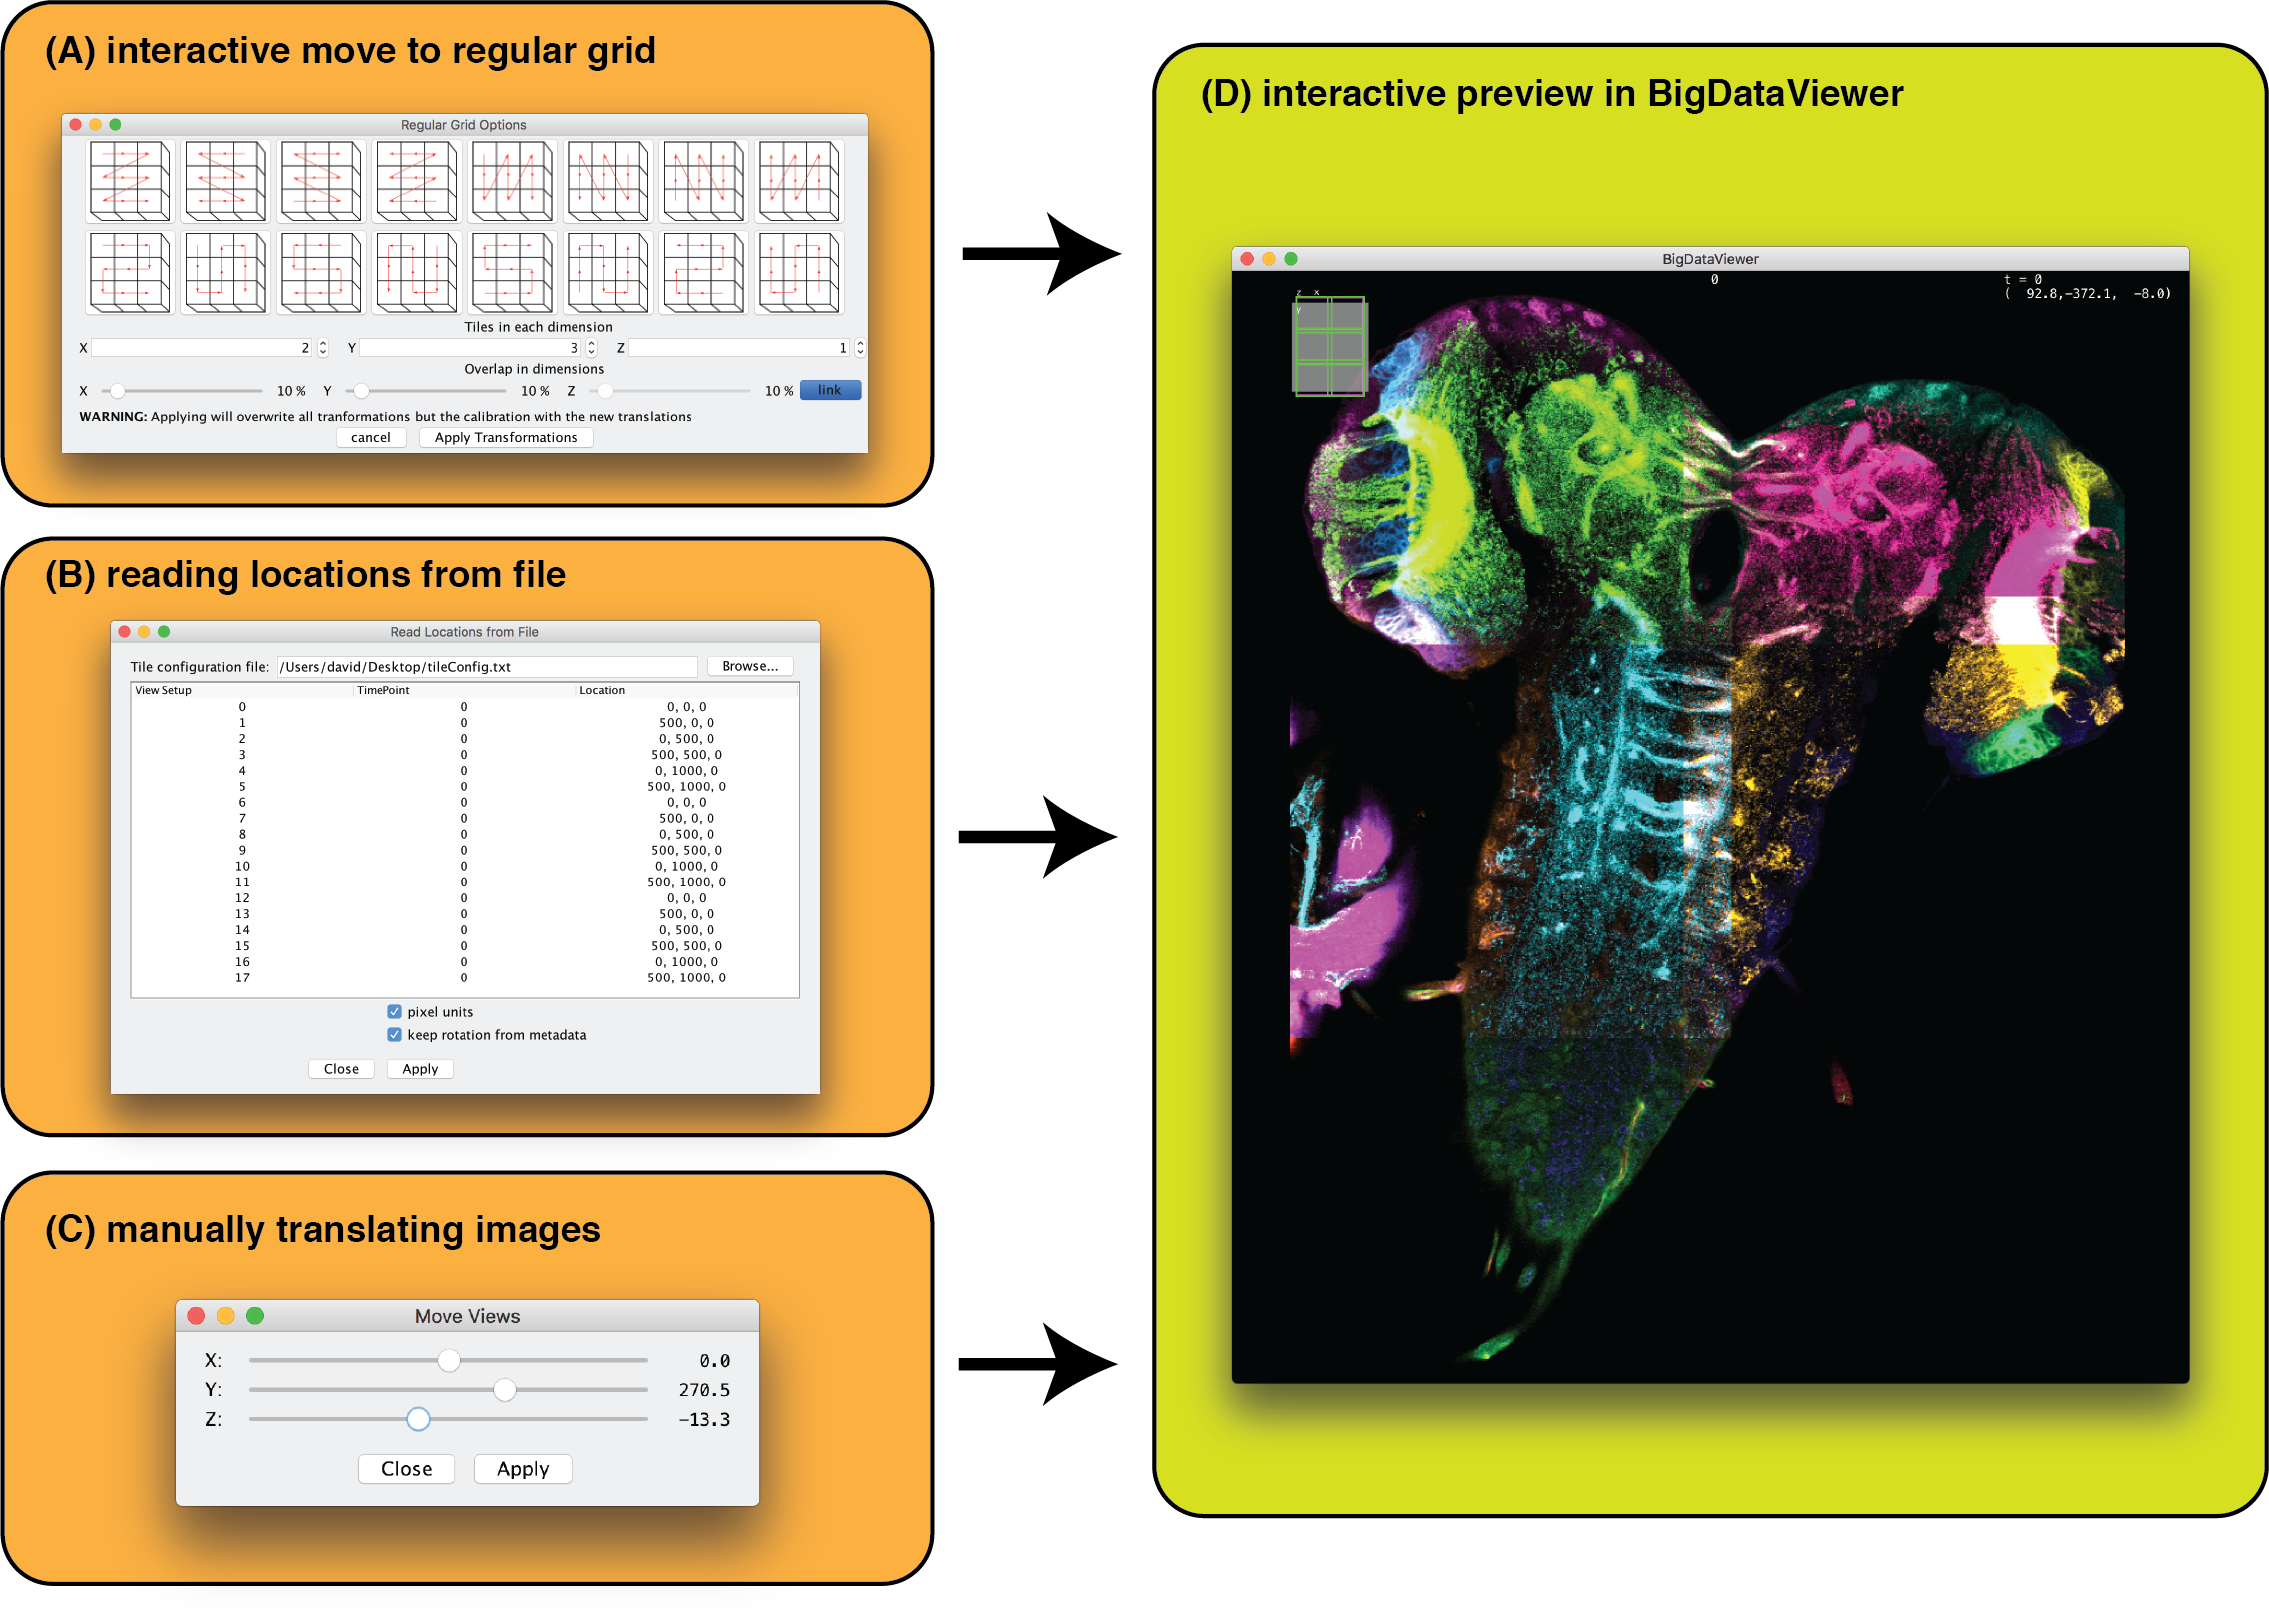
\includegraphics[width=\textwidth]{manual-view-arrangement.png}
\vspace{-2.0mm}
\caption{\hspace{-0.5mm} \emph{Interactive manual alignment of tiled images.} The BigStitcher GUI offers various ways of manually (pre-)aligning tiled images. Images can be moved to a regular grid with a given tile order and overlap \textbf{(A)}. Image locations can also be read from a simple \emph{tile configuration} text file \textbf{(B)}. Furthermore, selected image(s) can be moved along axes via sliders \textbf{(C)}. All changes will be displayed in the BigDataViewer window immediately \textbf{(D)} for quick verification. 
}
\label{fig:sup-fig-manual-align1}
\end{figure*}

\pagebreak

\subsection*{SUPPLEMENTARY FIGURE 4: Flat-field correction}
\vspace{1mm}
\begin{figure*}[h!]
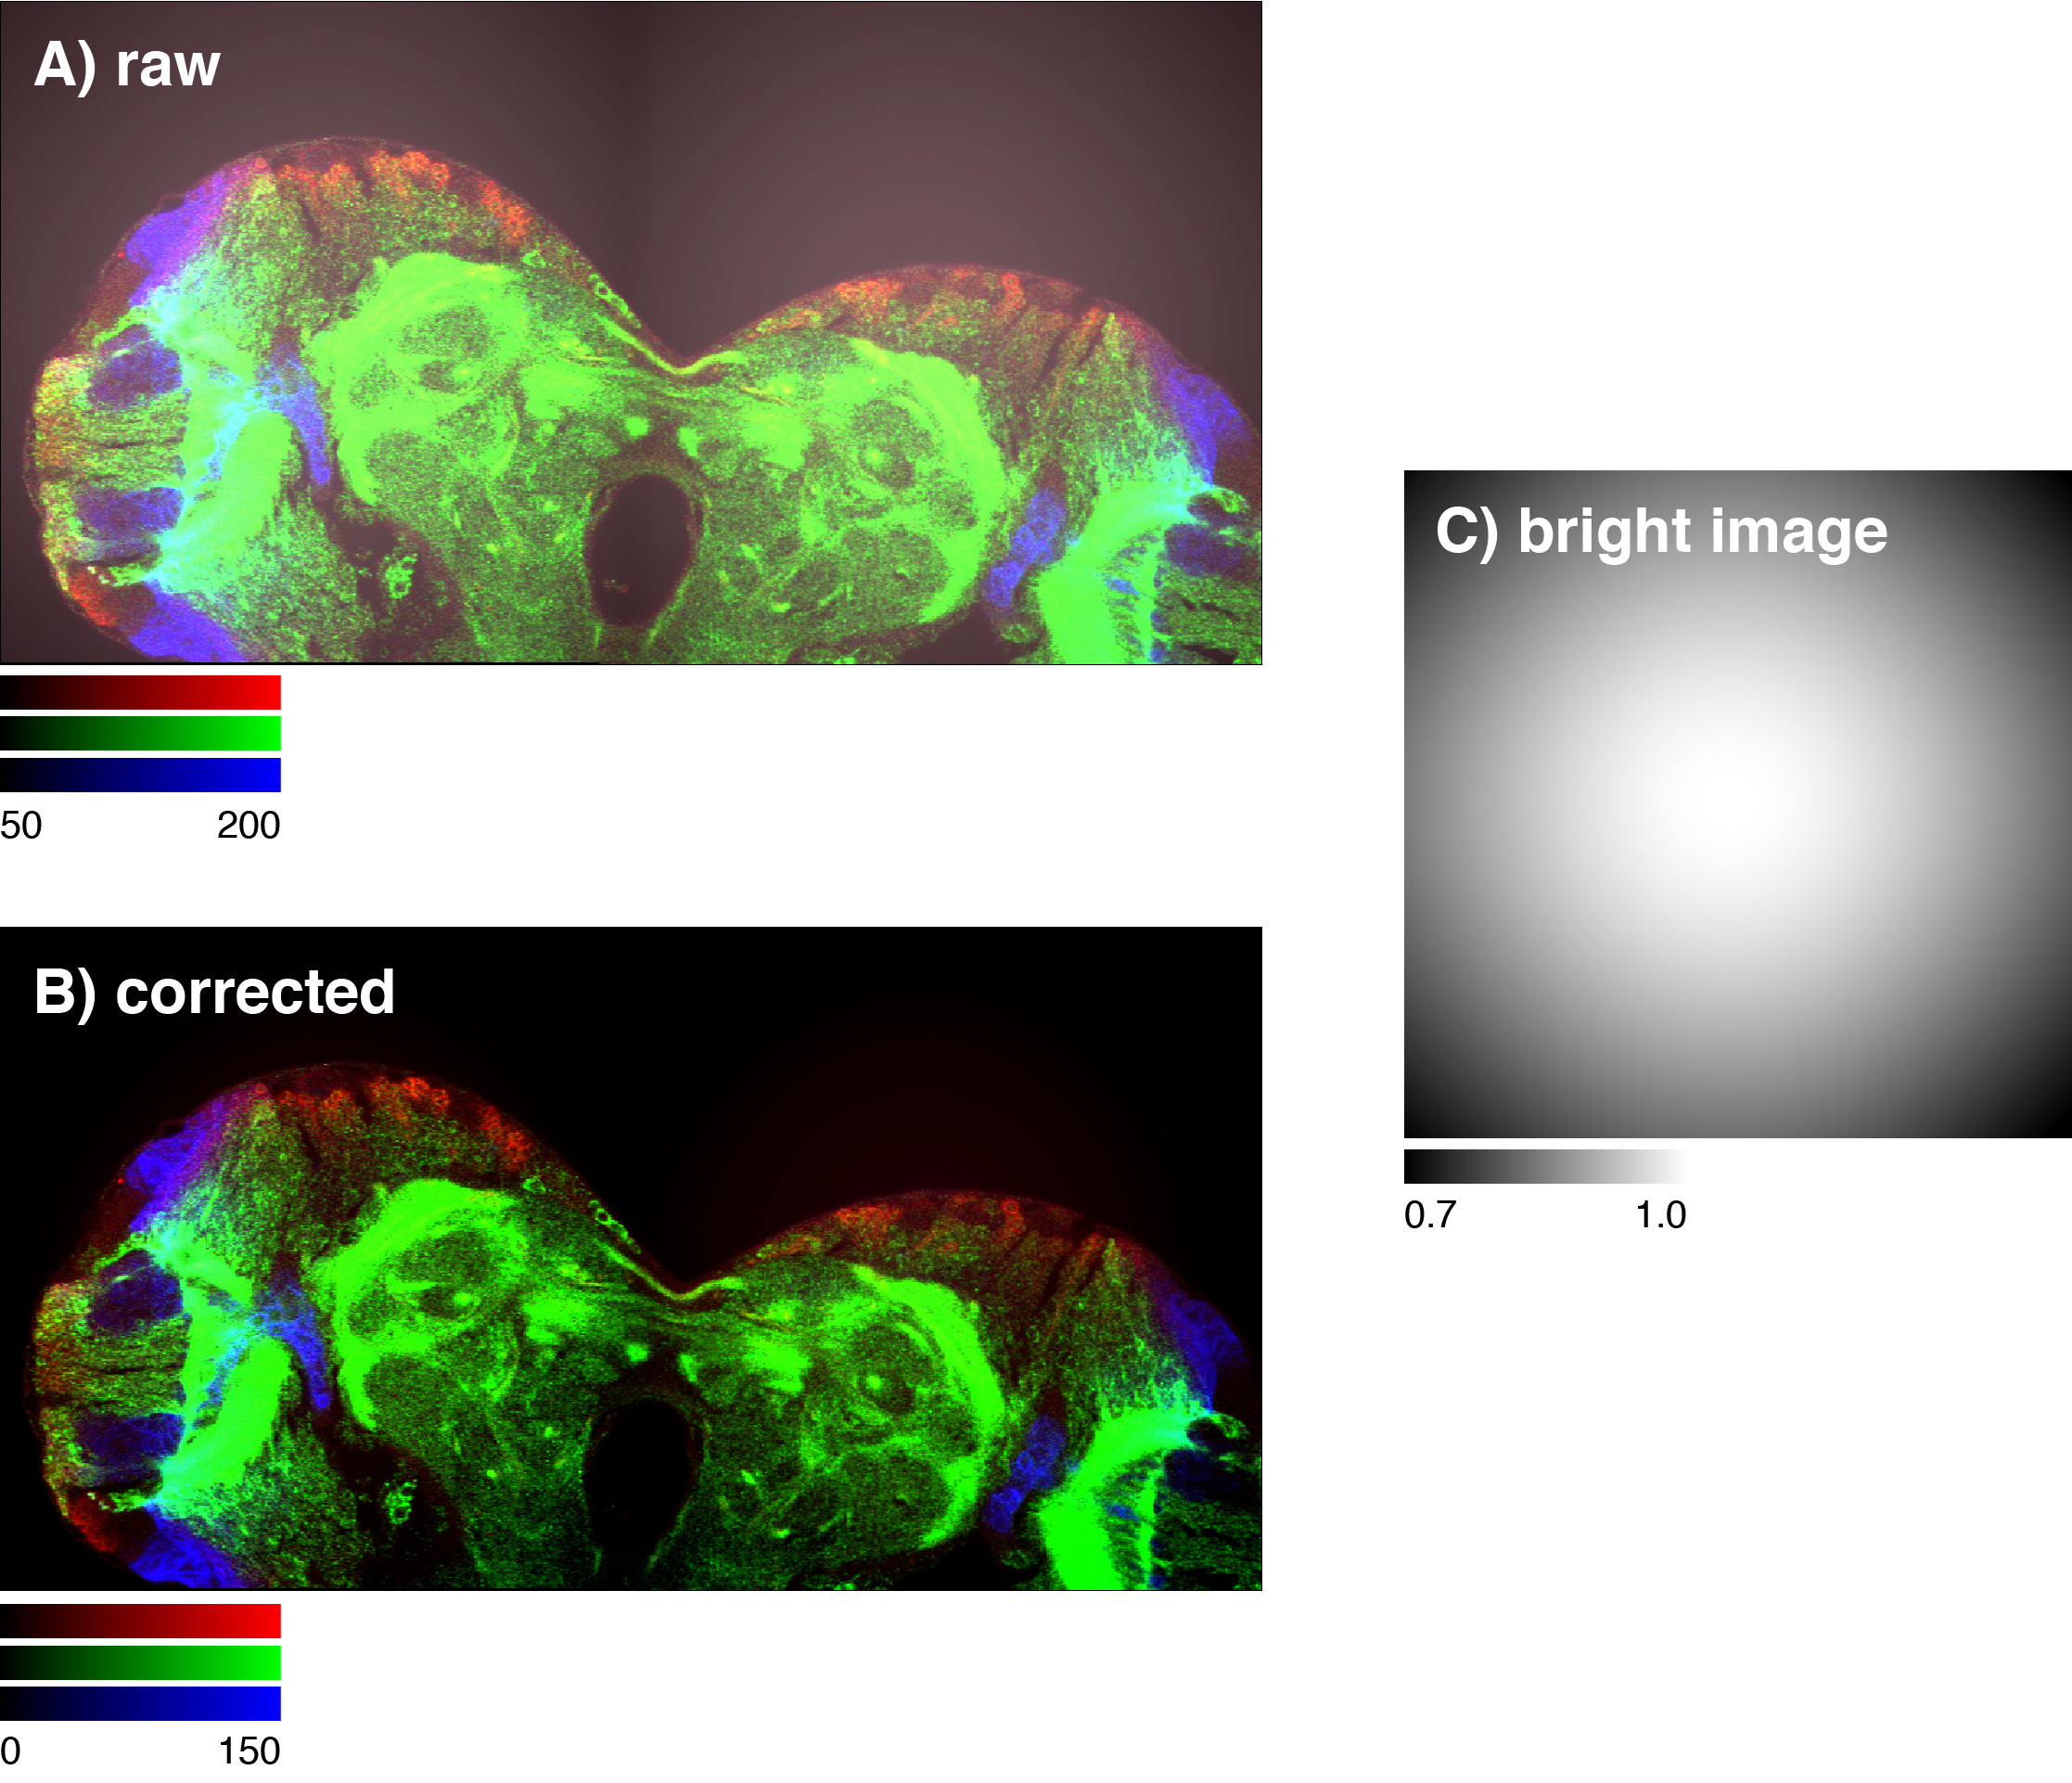
\includegraphics[width=\textwidth]{fig-flatfield.png}
\vspace{-2.0mm}
\caption{\hspace{-0.5mm} \emph{On-the-fly flat-field correction.} The BigStitcher offers correction for camera offsets, fixed pattern noise or uneven illumination. \textbf{(A)}  Simulation of the effects of a constant background offset and Gaussian illumination/detection efficiency \textbf{(C)} on tiled images. By subtracting the \emph{dark image} and modulating with the inverse relative intensity of the \emph{bright image}, such artifacts can be corrected easily \textbf{(B)}. The correction is calculated virtually, with optional caching, to allow for immediate inspection of the results.
}
\label{fig:sup-fig-flatfield}
\end{figure*}

\pagebreak

\subsection*{SUPPLEMENTARY FIGURE 5: Global optimization}
\vspace{1mm}
\begin{figure*}[h!]
\centerline{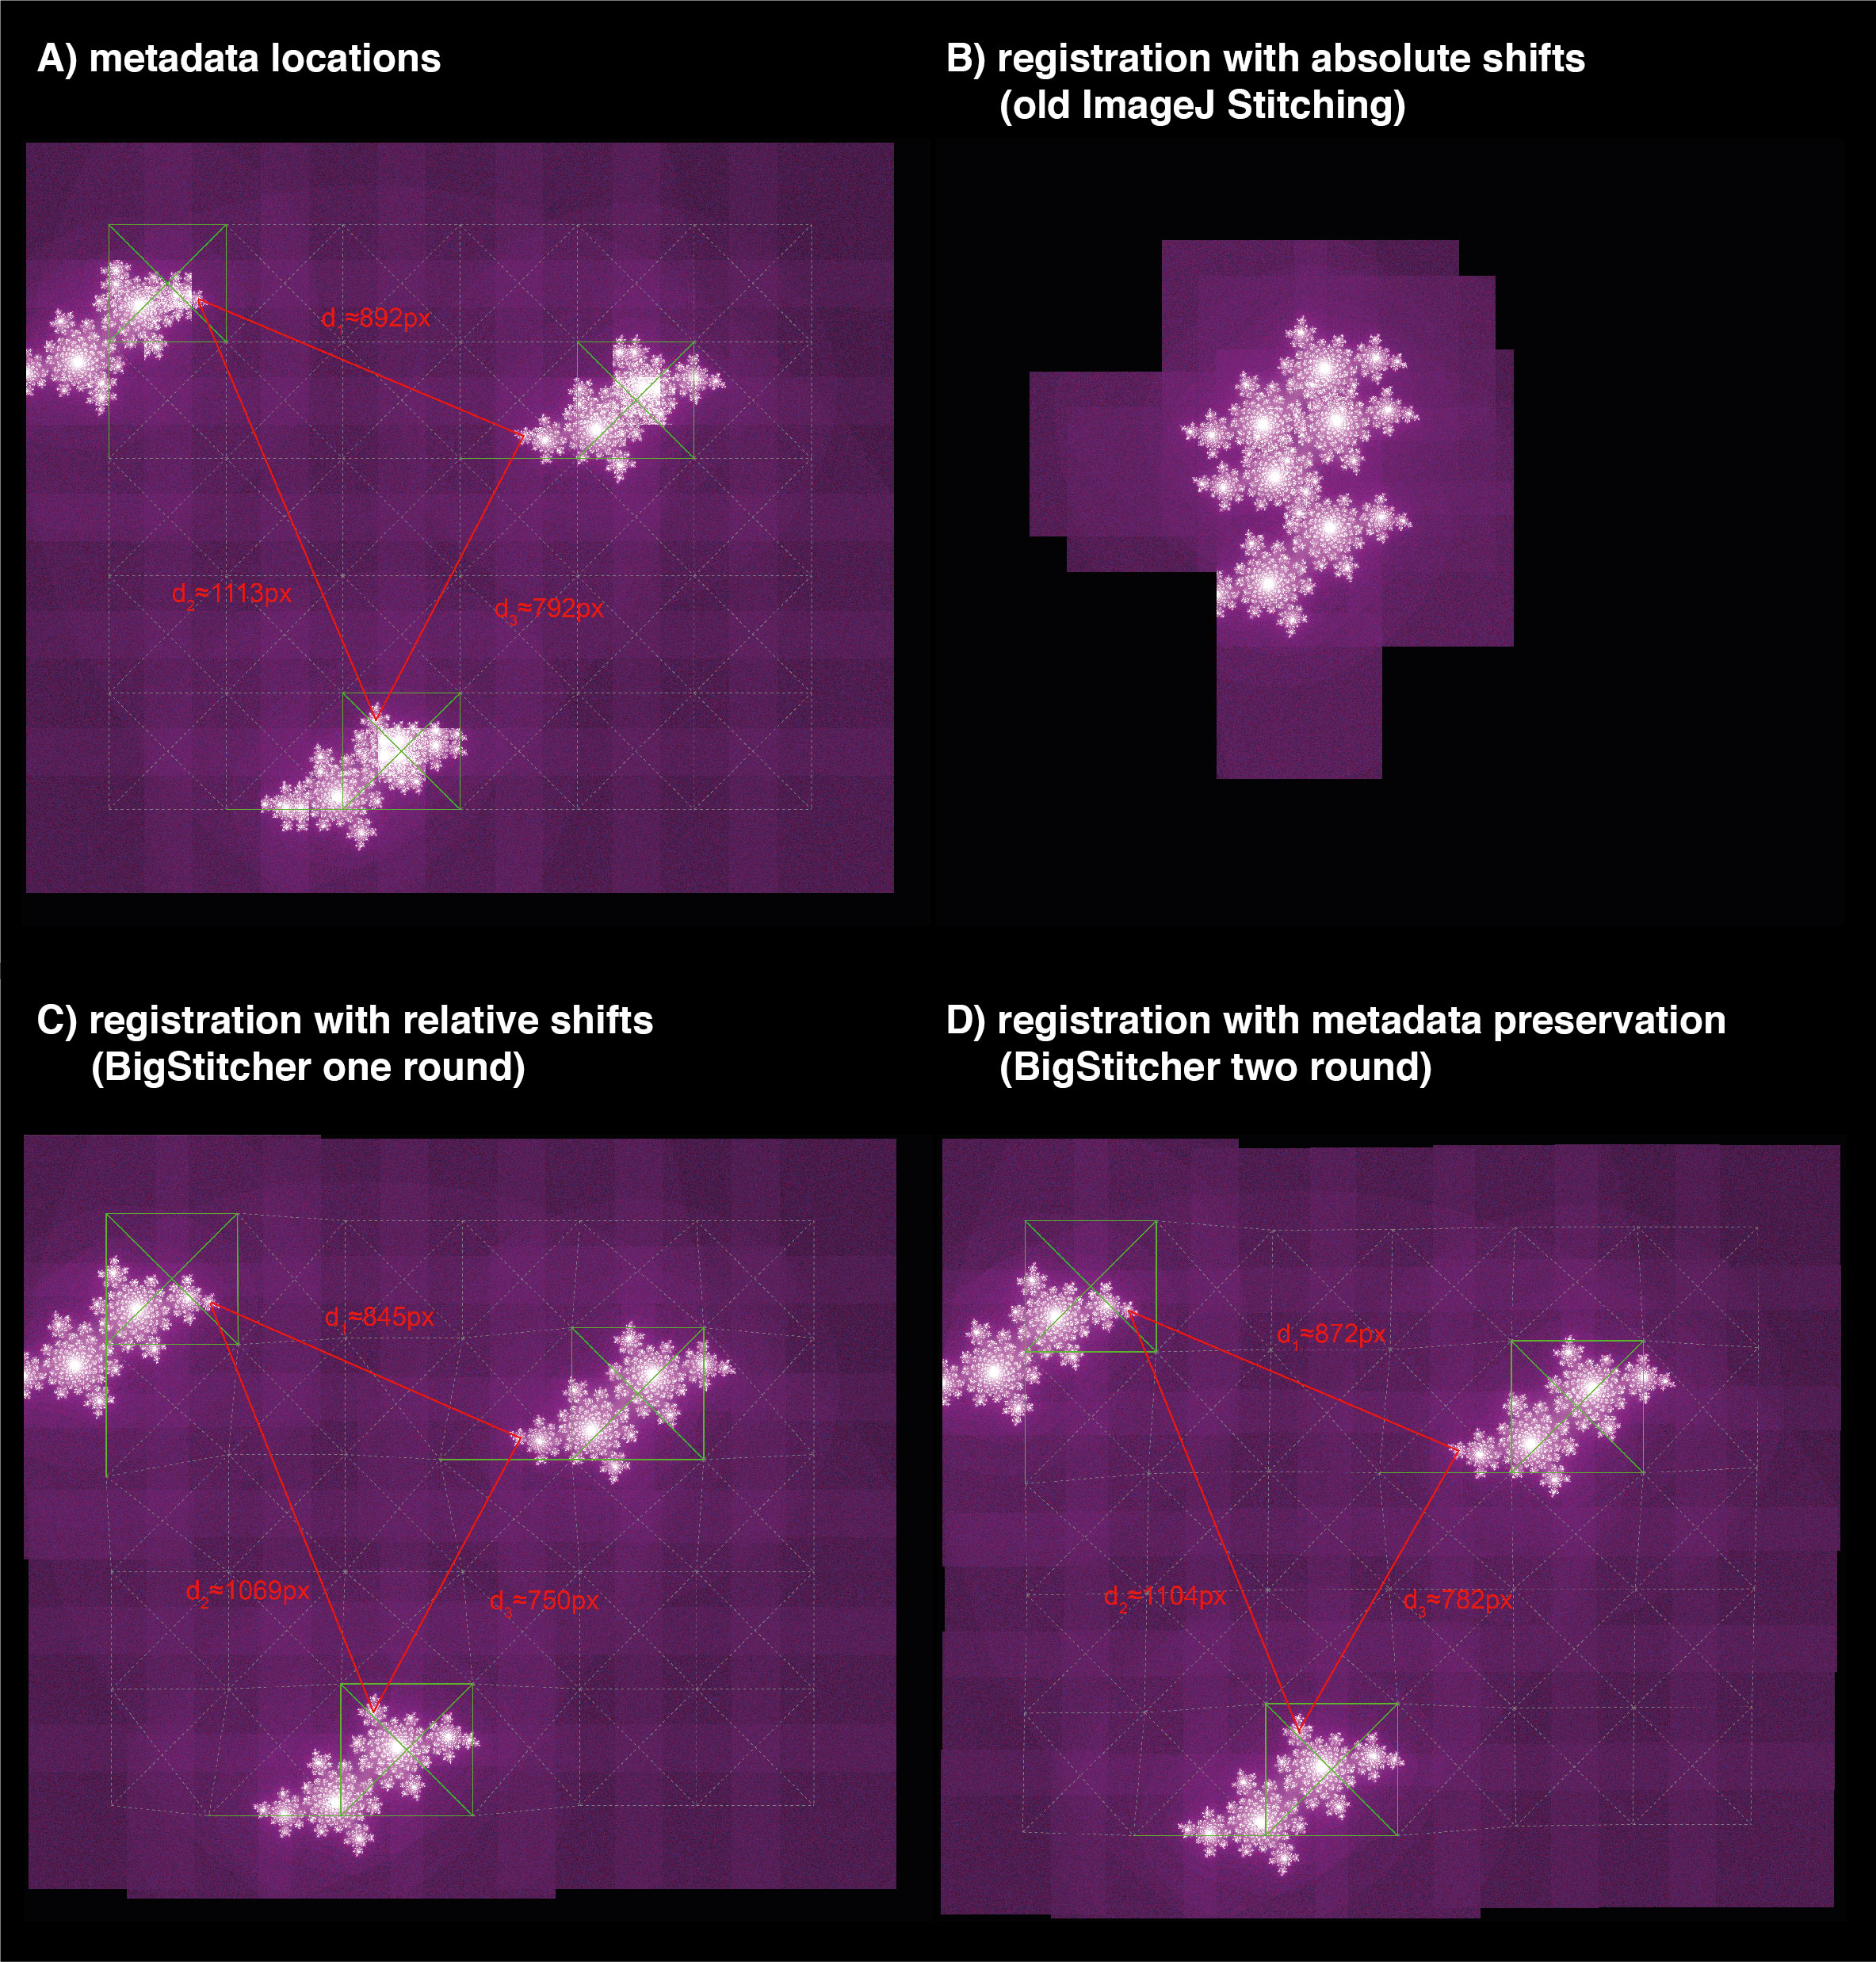
\includegraphics[width=0.85\textwidth]{fig-globalopt.png}}
\vspace{2.0mm}
\caption{\hspace{-0.5mm} \emph{Global optimization of pairwise registration in sparse datasets connected by "empty tiles" (noise only) .} \textbf{(A)} Simulation of a tiled image dataset with sparse objects: tiled images of multiple translated Julia fractals moved to a grid according to approximate metadata (with too high overlap). Centers of images for which pairwise shifts can be determined via phase correlation are connected by green lines, whereas centers of neighboring tiles for which no meaningful shift can be calculated are linked by dashed grey lines. Manually measured distances between distinct points in the three fractals are shown in red. Performing global optimization with \emph{absolute shifts} (as it is done BigStitcher's predecessor, the ImageJ Stitching plugin) will correctly align images within connected components of the link graph but place all fractals close to the origin \textbf{(B)}. By using \emph{relative shifts}, BigStitcher will leave disconnected objects at their initial location while still aligning within connected components \textbf{(C)}. As registrations are not propagated between unconnected tiles, distances between neighboring objects might change. By running a second round of optimization to align connected components according to metadata shifts and applying the results to the in-component registrations, distances between neighboring objects are preserved as-good-as-possible \textbf{(D)}.
}
\label{fig:sup-fig-globalopt}
\end{figure*}


\subsection*{SUPPLEMENTARY FIGURE 6: Pairwise registration by phase correlation}
\vspace{1mm}
\begin{figure*}[h!]
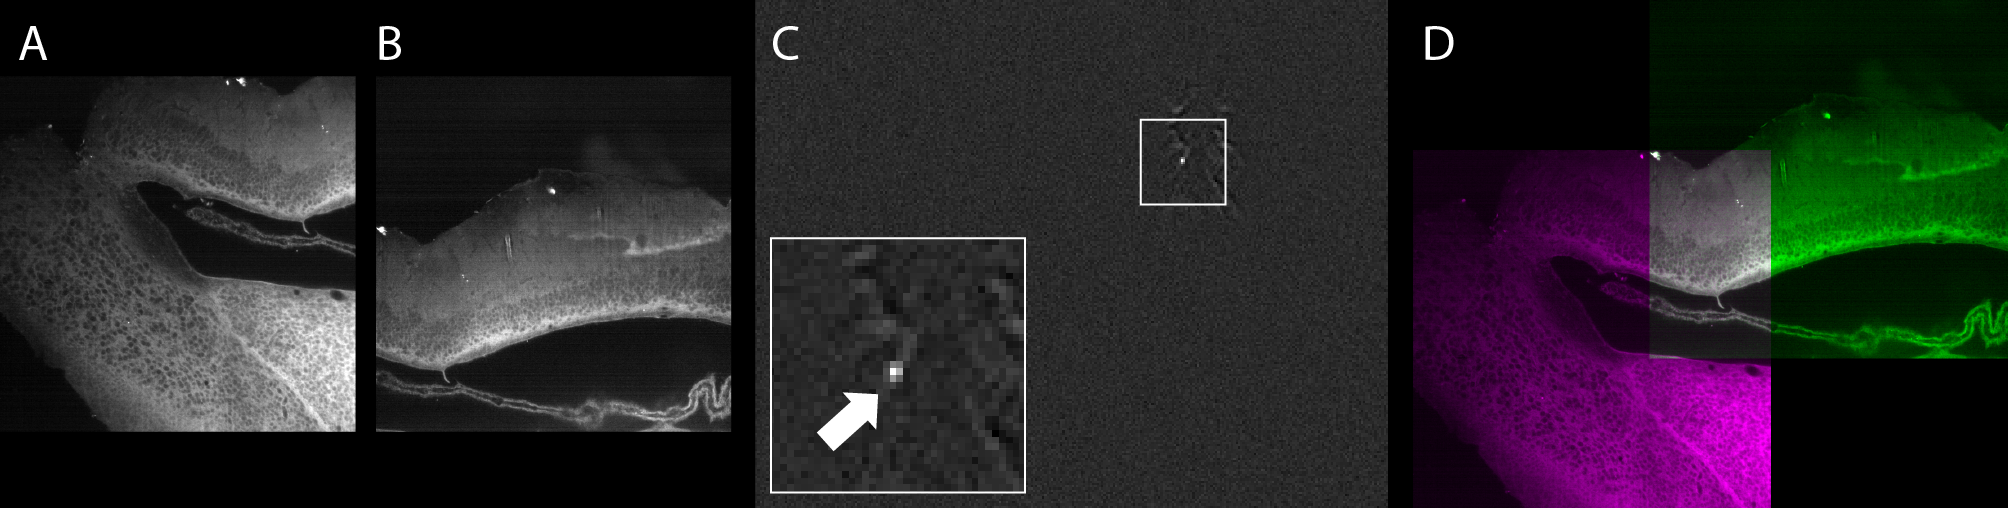
\includegraphics[width=\textwidth]{fig-stitching.png}
\vspace{-2.0mm}
\caption{\hspace{-0.5mm} \emph{Pairwise registration by phase correlation}. \textbf{(A),(B)} Central slices of image stacks from a tiled acquisition (non-regular tiling) of an adult mouse hypothalamus slice. \textbf{(C)} Phase correlation matrix (PCM) calculated from the two images shows a single, distinct peak above nearly constant background. The peak location corresponds to the relative translation $t$ of both tiles. \textbf{(D)} Central slice through the images aligned according to $t$, as displayed in interactively during the reconstruction process. 
}
\label{fig:sup-fig-stitching}
\end{figure*}

\subsection*{SUPPLEMENTARY FIGURE 7: Downsampling with different SNR}
\vspace{1mm}
\begin{figure*}[h!]
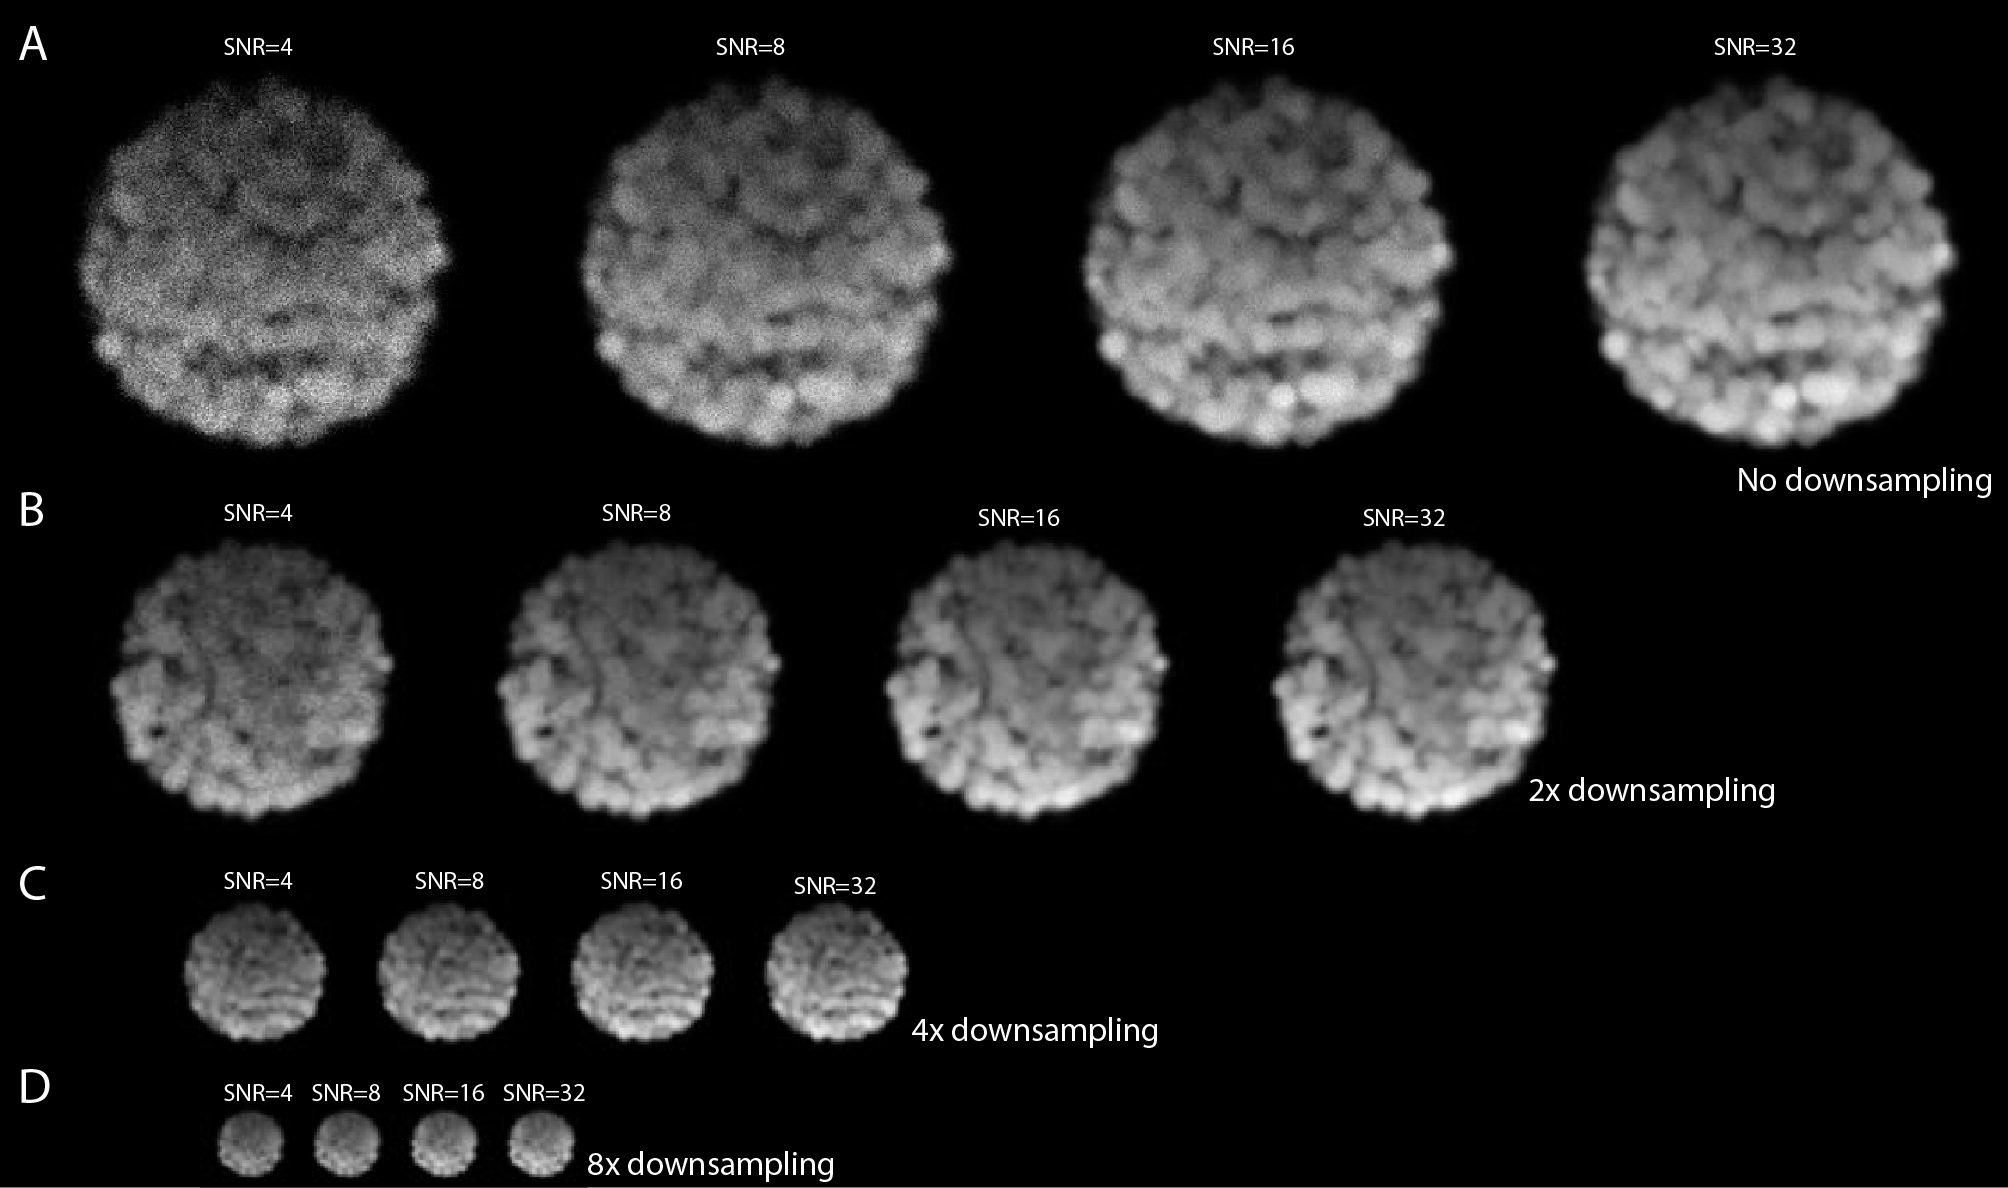
\includegraphics[width=\textwidth]{fig-downsampling.png}
\vspace{-2.0mm}
\caption{\hspace{-0.5mm} \emph{Effects of downsampling on simulated data with different SNR.} \textbf{(A)} Simulated image stacks of spheroid-like objects deteriorated by anisotropic sampling, light attenuation, convolution with an anisotropic PSF, and pixel intensity generation using Poisson processes to archive desired signal-to-noise-ratios (SNRs). A central slice through 3d volumes is shown. \textbf{(B), (C), (D)} Effects of downsampling on the simulated images. The effects of Poisson Shot Noise are gradually reduced by the blurring of increasing downsampling.
}
\label{fig:sup-fig-downsampling}
\end{figure*}

\pagebreak

\subsection*{SUPPLEMENTARY FIGURE 8: Downsampling statistics 1}
\vspace{1mm}
\begin{figure*}[h!]
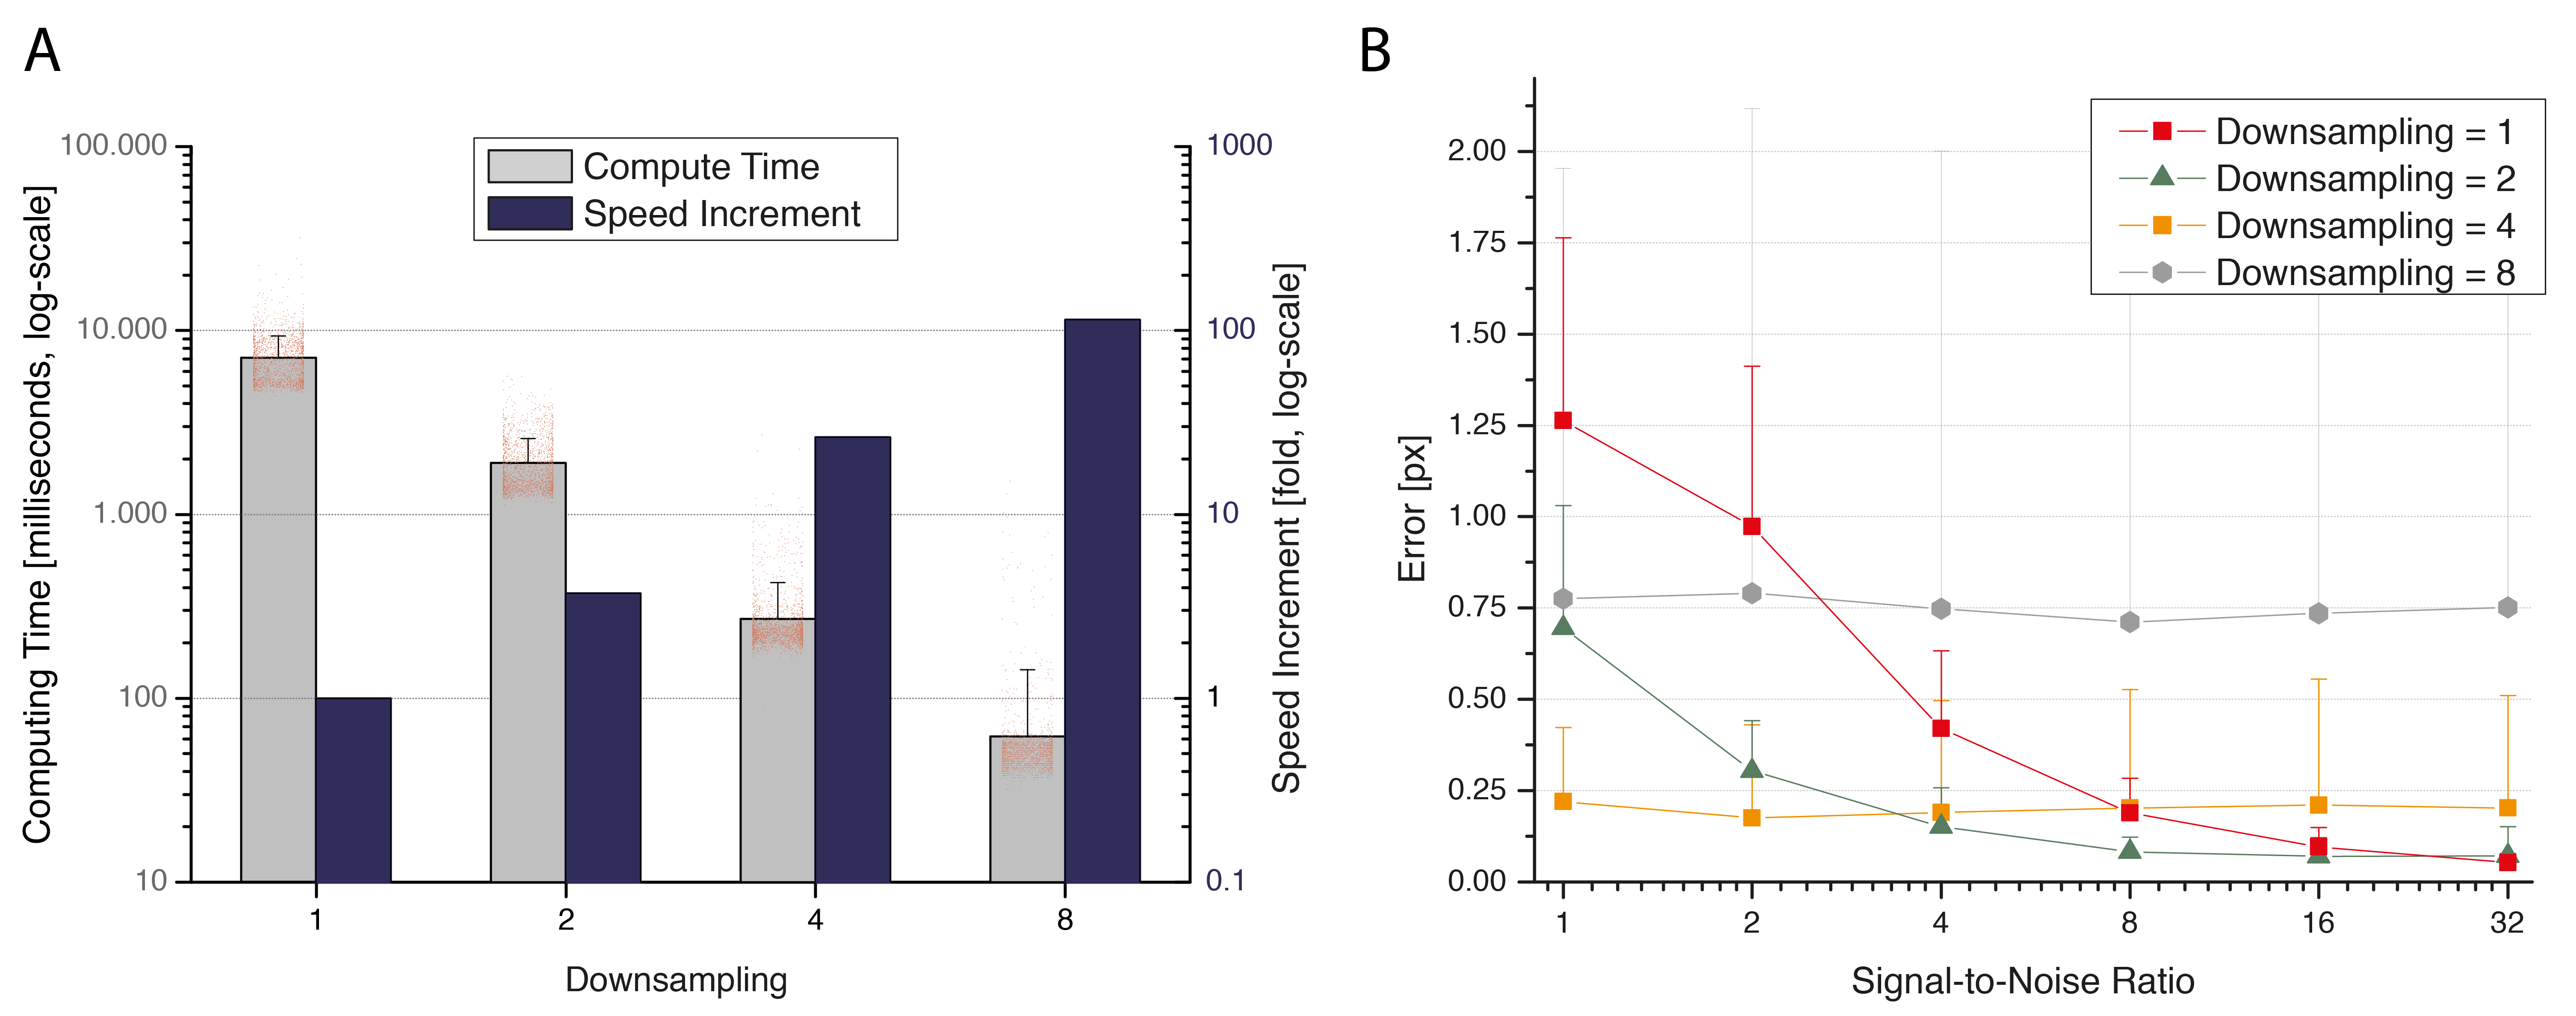
\includegraphics[width=\textwidth]{fig-downsampling-statistics-0.png}
\vspace{-2.0mm}
\caption{\hspace{-0.5mm} \emph{Processing times and overall errors.} \textbf{(A)} Processing times for sub-pixel precise identification of overlap between simulation spheroids. With increasing downsampling, the computation time drops significantly. \textbf{(B)} Average errors including their standard deviation for all combinations of SNR and downsampling. \textbf{(A,B)} All errors are in units of the input images (no downsampling). For each combination of SNR and downsampling 300 independent simulations were run to compute the values.
}
\label{fig:sup-fig-downsampling-statistics-0}
\end{figure*}

\subsection*{SUPPLEMENTARY FIGURE 9: Downsampling statistics 2}
\vspace{1mm}
\begin{figure*}[h!]
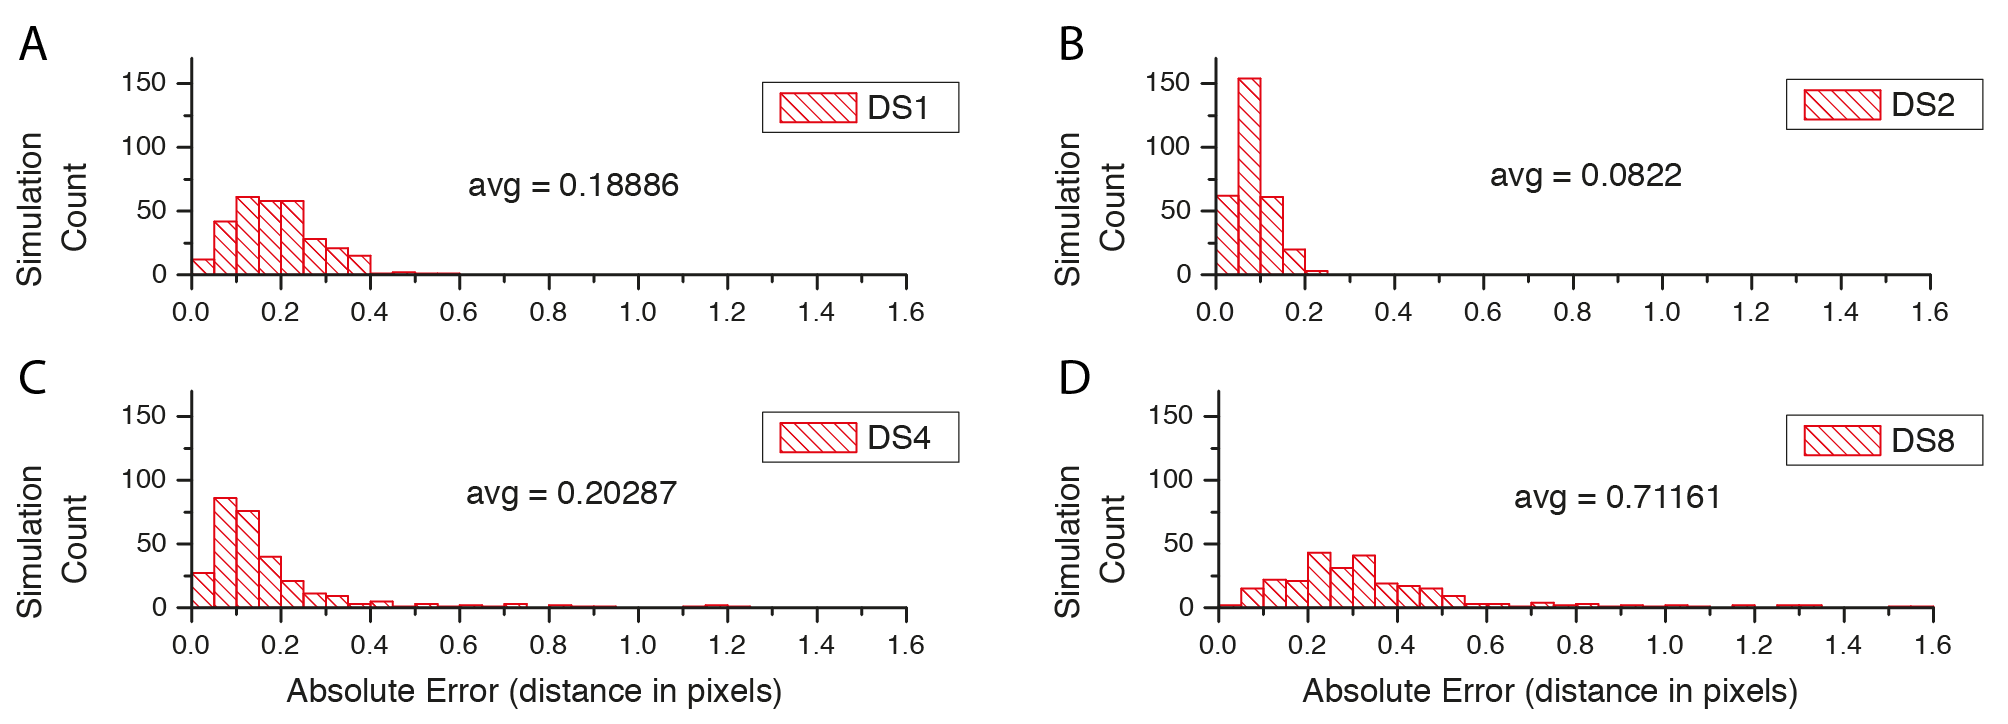
\includegraphics[width=\textwidth]{fig-downsampling-statistics-1.png}
\vspace{-2.0mm}
\caption{\hspace{-0.5mm} \emph{Errors for different downsamplings at SNR=8.} \textbf{(A-D)} Histograms showing the distributions of error of the simulations. Errors initially decrease due to the smoothing effect of the downsampling. All errors are in pixel units of the original resolution (DS1). Each histogram consists of 300 independent simulations.
}
\label{fig:sup-fig-downsampling-statistics-1}
\end{figure*}

\pagebreak

\subsection*{SUPPLEMENTARY FIGURE 10: Downsampling statistics 3}
\vspace{1mm}
\begin{figure*}[h!]
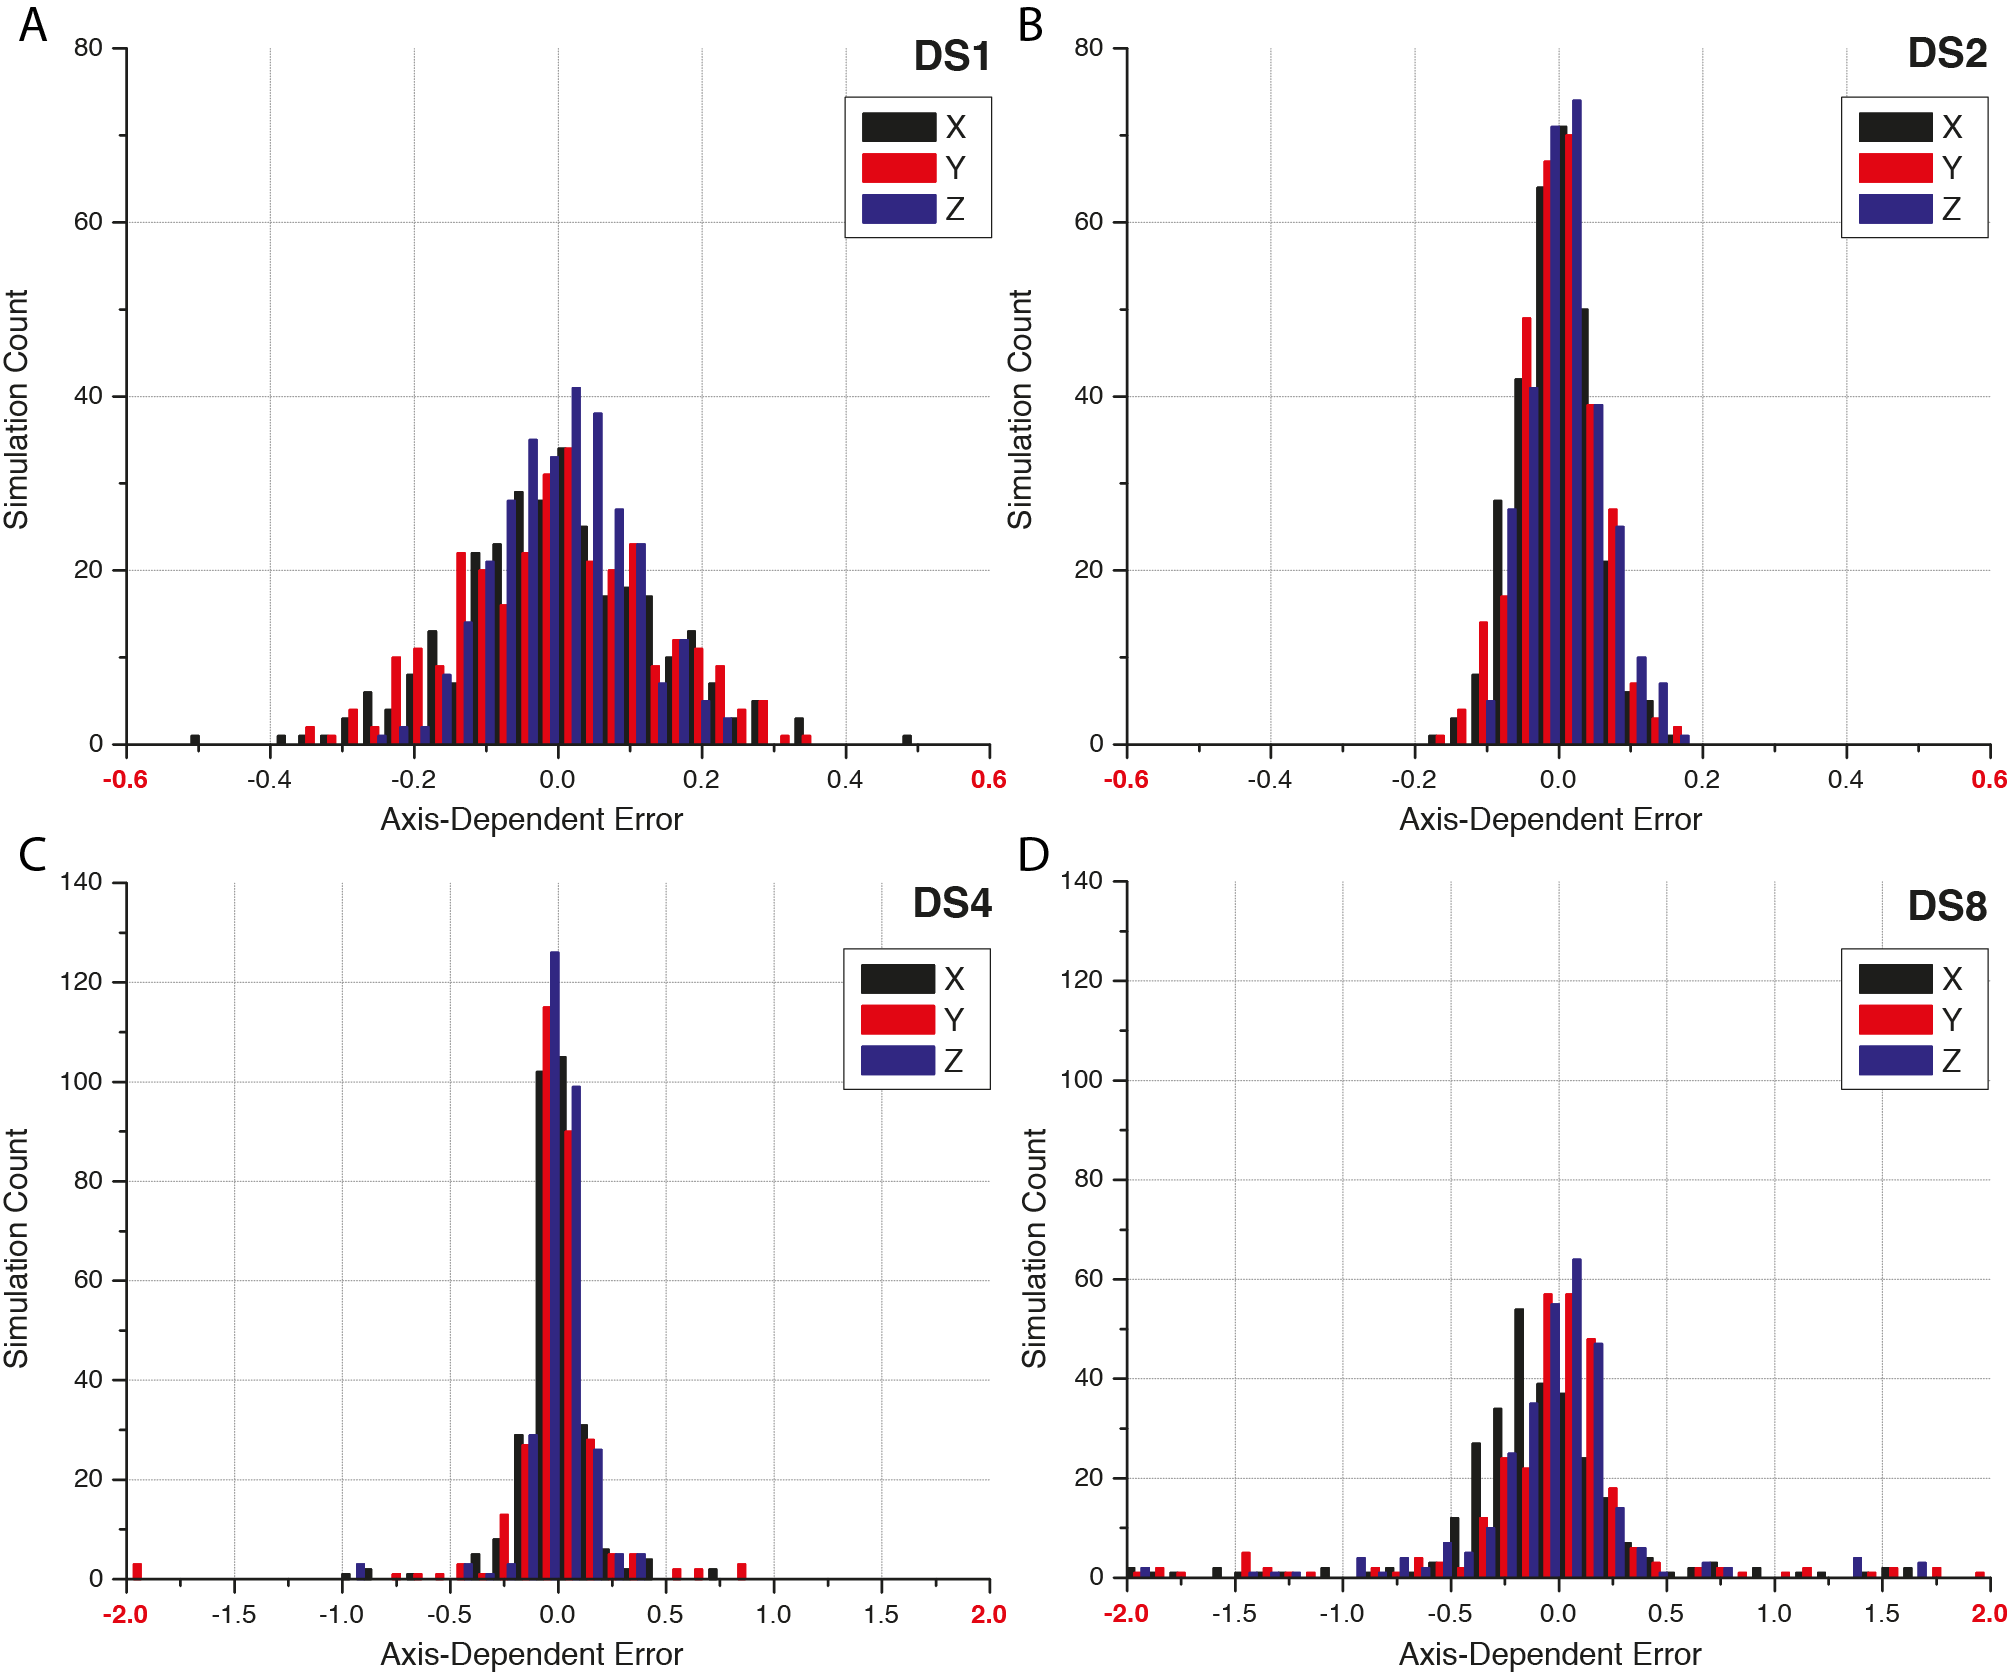
\includegraphics[width=\textwidth]{fig-downsampling-statistics-2.png}
\vspace{-2.0mm}
\caption{\hspace{-0.5mm} \emph{Absolute distance errors at SNR=8.} \textbf{(A-D)}  Histograms showing the absolute distances between computed and know shift between two simulated spheroids, split by dimension. It illustrates a normal distribution of the error made during the pairwise phase correlation. All errors are in pixel units of the original resolution (DS1). Each histogram consists of 300 independent simulations.
}
\label{fig:sup-fig-downsampling-statistics-2}
\end{figure*}

\pagebreak

\subsection*{SUPPLEMENTARY FIGURE 11: Interactive inspection and curation of pairwise links}
\vspace{1mm}
\begin{figure*}[h!]
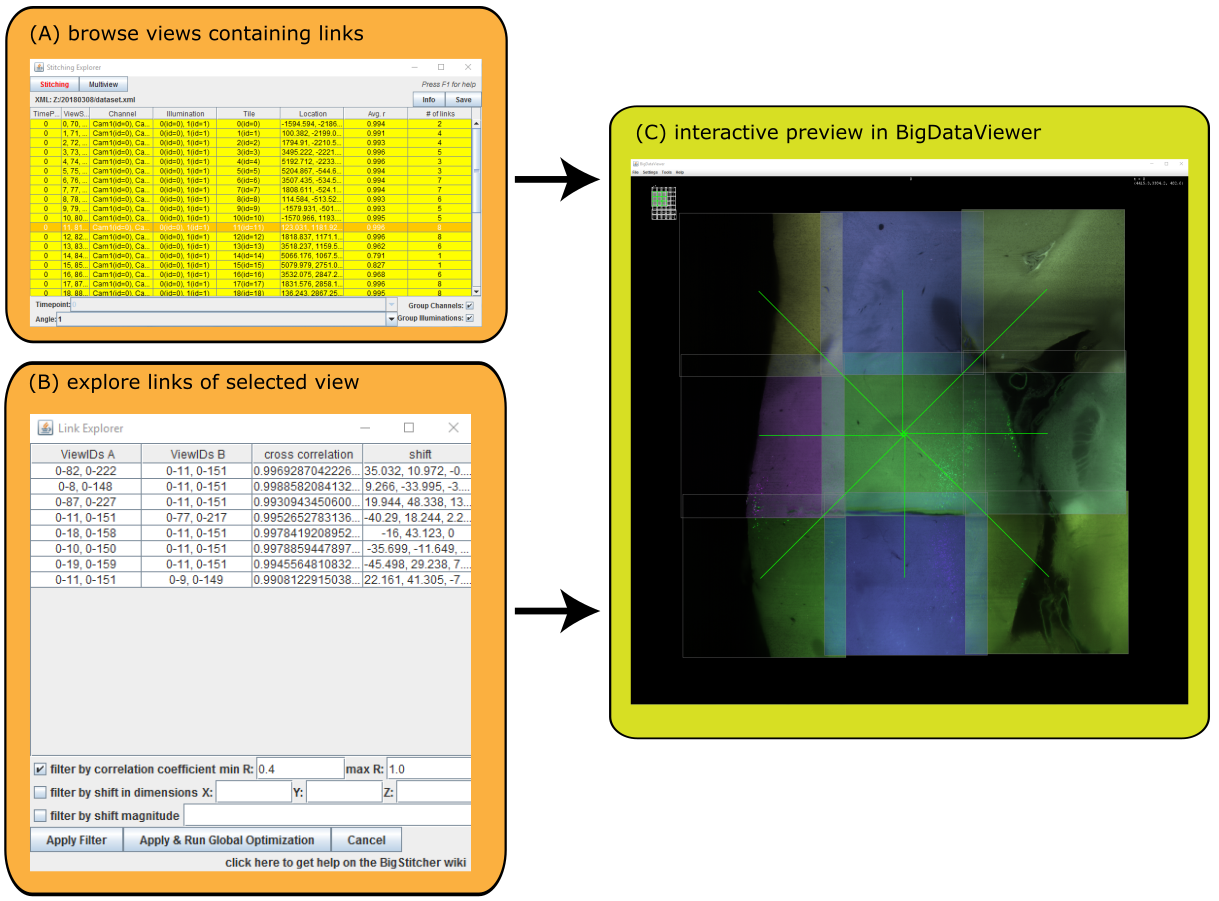
\includegraphics[width=\textwidth]{Supp-Link-Explorer.png}
\vspace{-2.0mm}
\caption{\hspace{-0.5mm} \emph{Interactive visualization of links in the link explorer.} The BigStitcher GUI offers the exploring and modifying calculated links between corresponding tiles in the link explorer menu. \textbf{(A)} Tiles containing links are displayed in yellow and can be selected. \textbf{(B)} Display corresponding tiles of the selected view. Single links can be removed manually or through available filtering options. \textbf{(C)} Corresponding links of the selected view are displayed in real-time in the BigDataViewer.
}
\label{fig:sup-fig-link-explorer}
\end{figure*}

\pagebreak


\subsection*{SUPPLEMENTARY FIGURE 12: Affine refinement via ICP}
\vspace{1mm}
\begin{figure*}[h!]
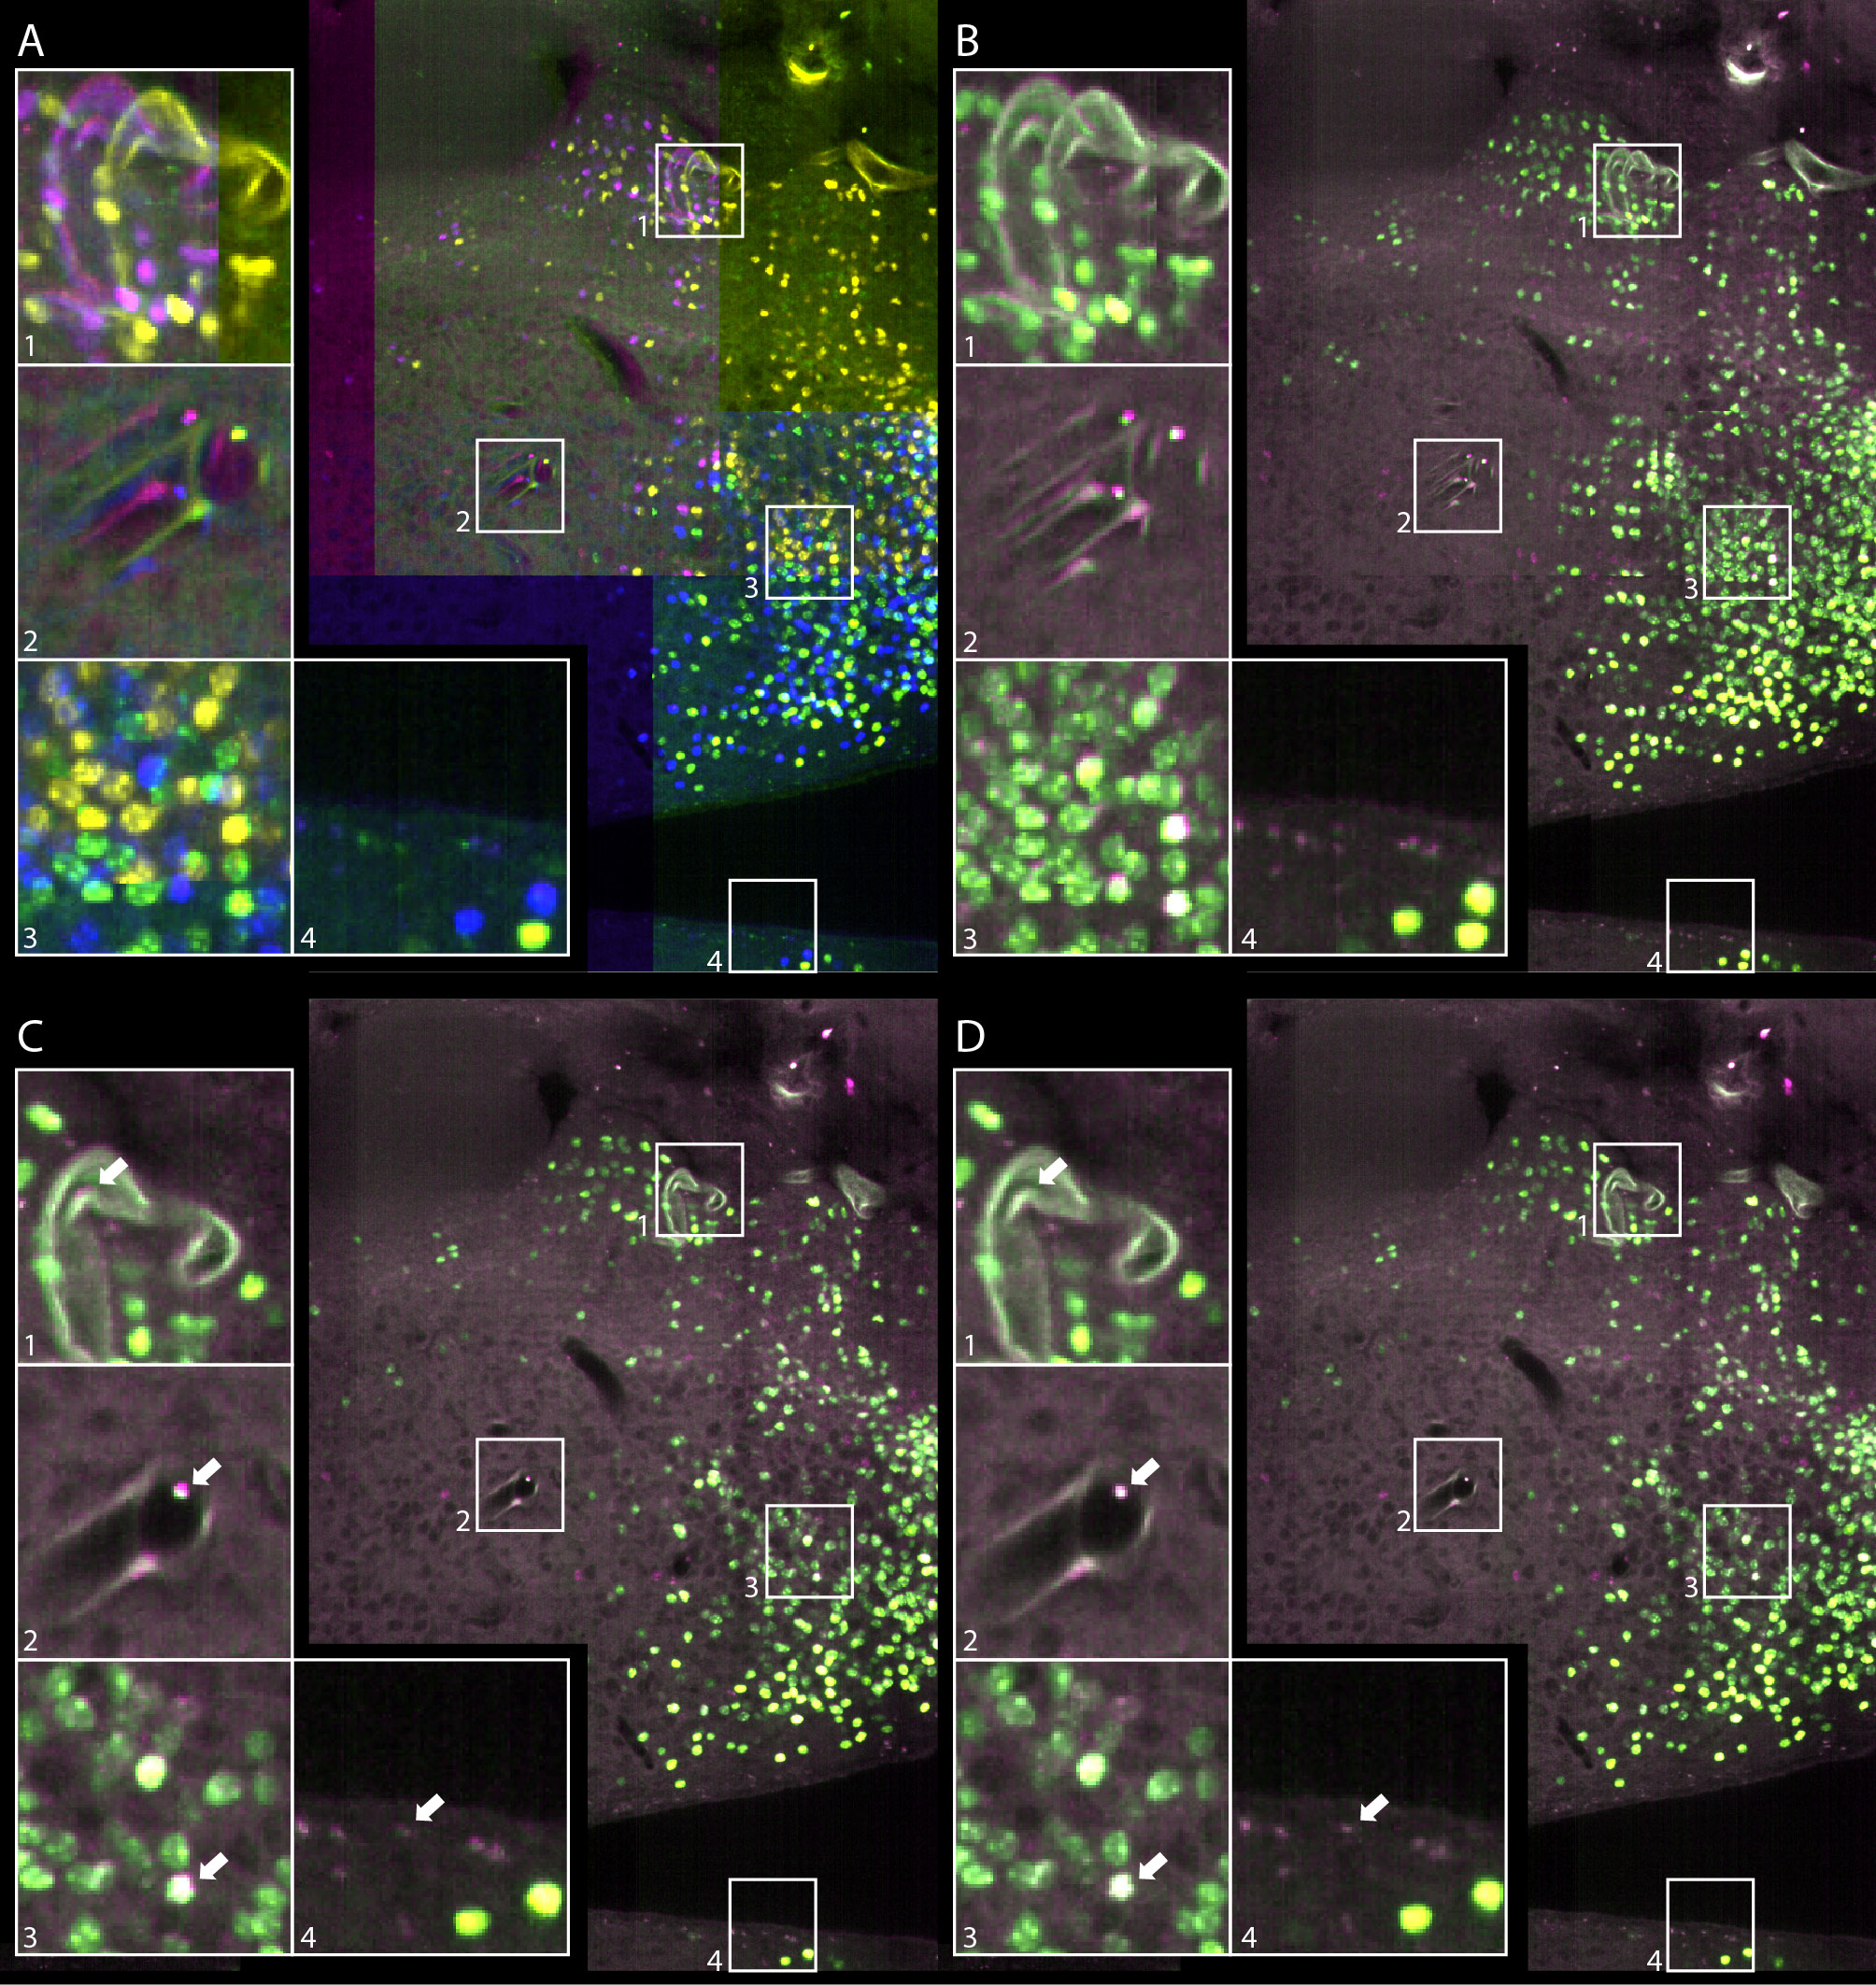
\includegraphics[width=\textwidth]{fig-stitching_icp.png}
\vspace{-2.0mm}
\caption{\hspace{-0.5mm} \emph{Illustration of different steps for multi-tile alignment} \textbf{(A)} Four overlapping image tiles randomly color-coded illustrate the typical error when only the metadata as read from the microscope is applied. \textbf{(B)} Shows the same four image tiles as in (A), but without random color coding. \textbf{(C)} Quality of the registration after applying the phase-correlation based stitching with downsampling 4 and two-round global optimization. \textbf{(D)} Result after applying the automatic ICP refinement for tile alignment and chromatic aberration correction. \textbf{(A-D)} Insets highlight specific areas to better appreciate quality differences.
}
\label{fig:sup-fig-icp}
\end{figure*}

\pagebreak

\subsection*{SUPPLEMENTARY FIGURE 13: Bounding Box definition}
\vspace{1mm}
\begin{figure*}[h!]
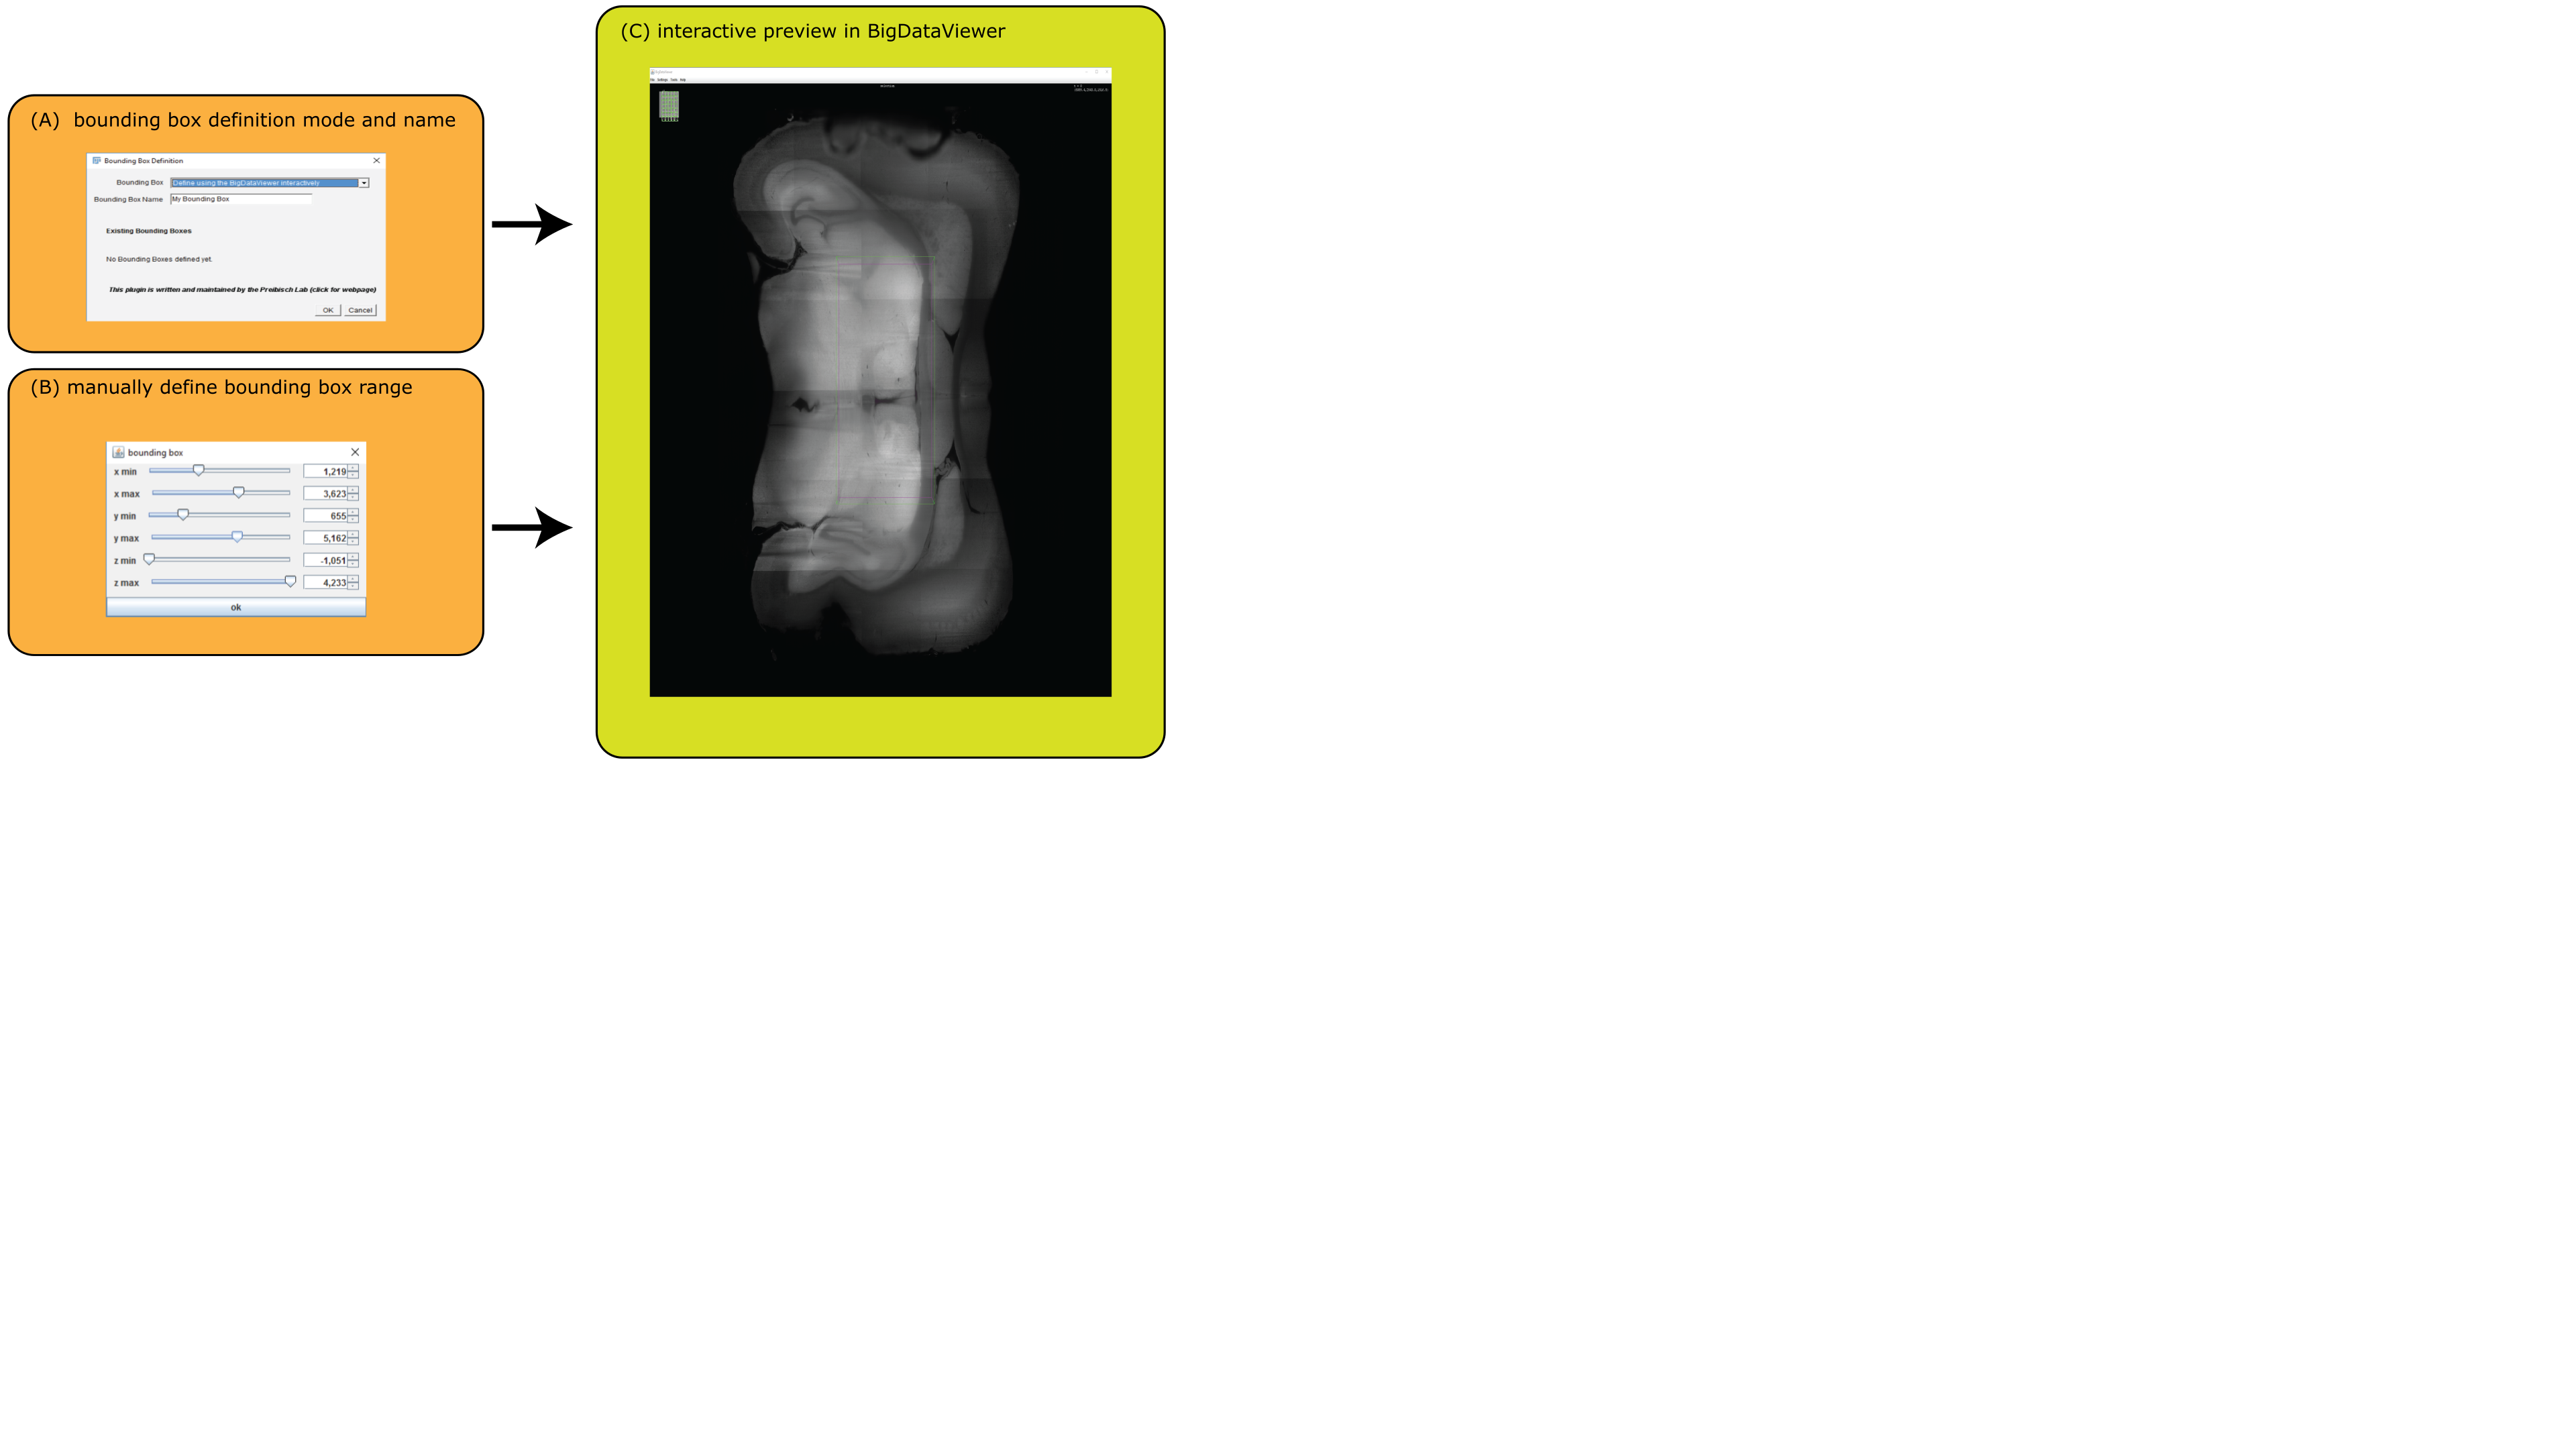
\includegraphics[width=\textwidth]{Supp-BB.png}
\vspace{-2.0mm}
\caption{\hspace{-0.5mm} \emph{Interactive definition of bounding boxes.} The BigStitcher GUI offers the possibility of defining or modifying regions of interest via the creation of bounding boxes. \textbf{(A)} Choose the method used to define a new bounding box. In this case the interactive mode is selected. \textbf{(B)} manually define the bounding box range \textbf{(C)} Preview the size of the specified bounding box in the BigDataViewer in real-time.
}
\label{fig:sup-fig-boundingbox}
\end{figure*}

\pagebreak


\subsection*{SUPPLEMENTARY FIGURE 14: Virtual Fusion of large image}
\vspace{1mm}
\begin{figure*}[h!]
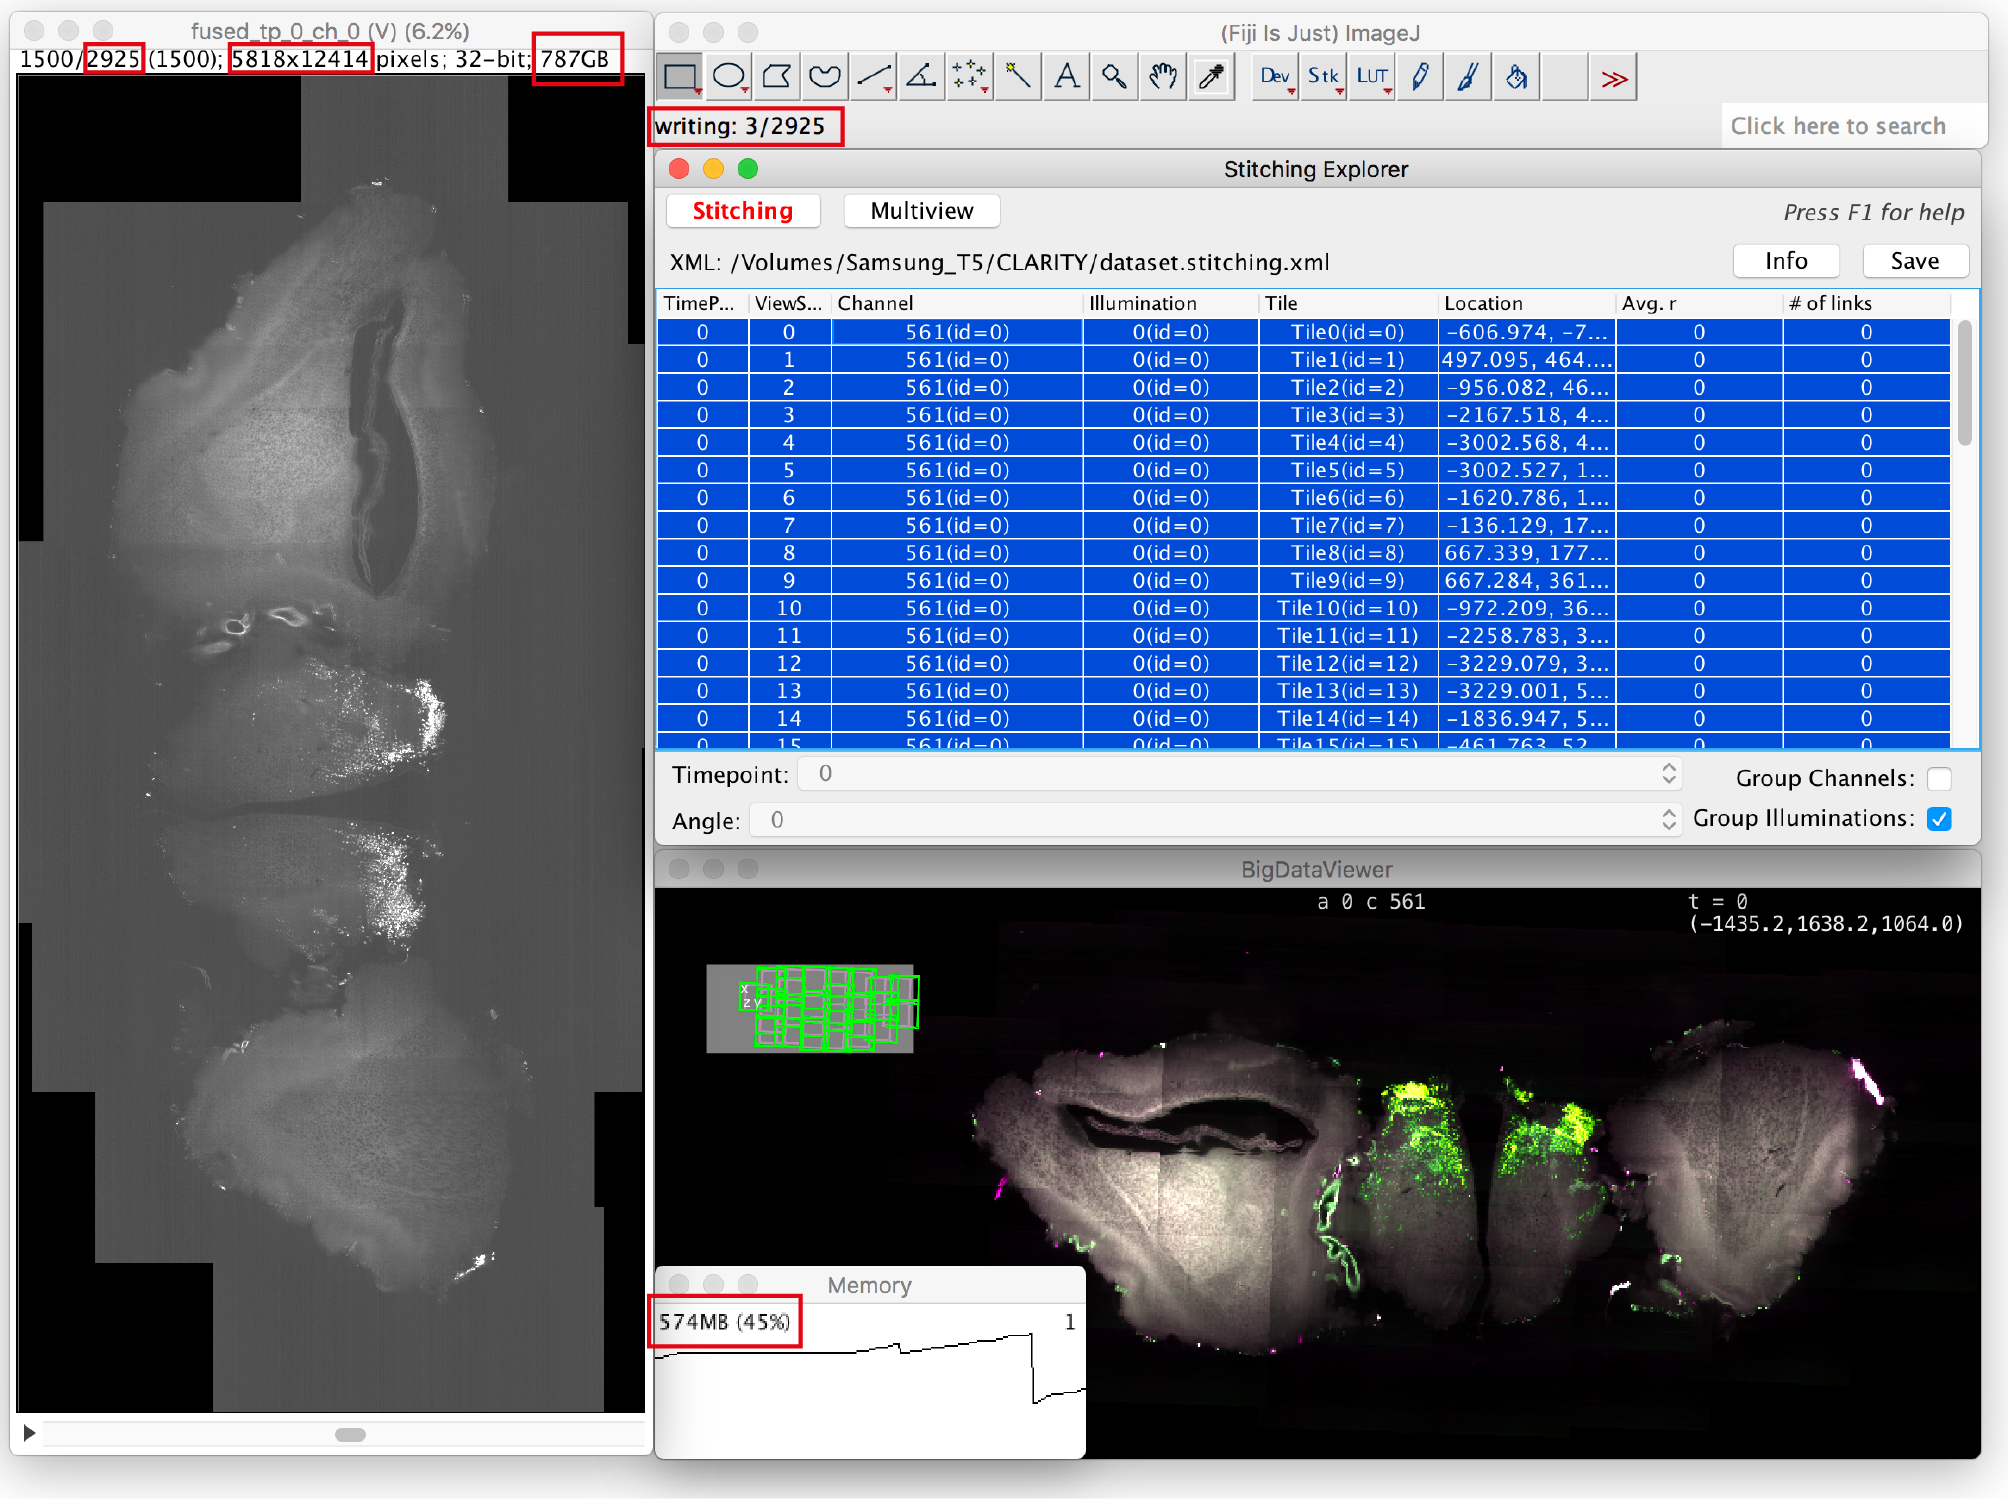
\includegraphics[width=\textwidth]{fig-fusion-screenshot.png}
\vspace{-2.0mm}
\caption{\hspace{-0.5mm} \emph{Virtual Fusion.} Screenshot of a Fiji instance running with \textbf{1.25GB of RAM} successfully fusing and saving a \textbf{787GB} volume 5818$\times$12414$\times$2925 pixels in size. This is achieved through \textbf{virtual fusion} combined with virtual, cached loading of blocked, multi-resolution input images. Red boxes highlight memory consumption, size, and progress. During the fusion process, the BigStitcher and BigDataViewer are interactively accessible.
}
\label{fig:sup-fig-fusion}
\end{figure*}

\pagebreak

\subsection*{SUPPLEMENTARY FIGURE 15: Interest point visualization}
\vspace{1mm}
\begin{figure*}[h!]
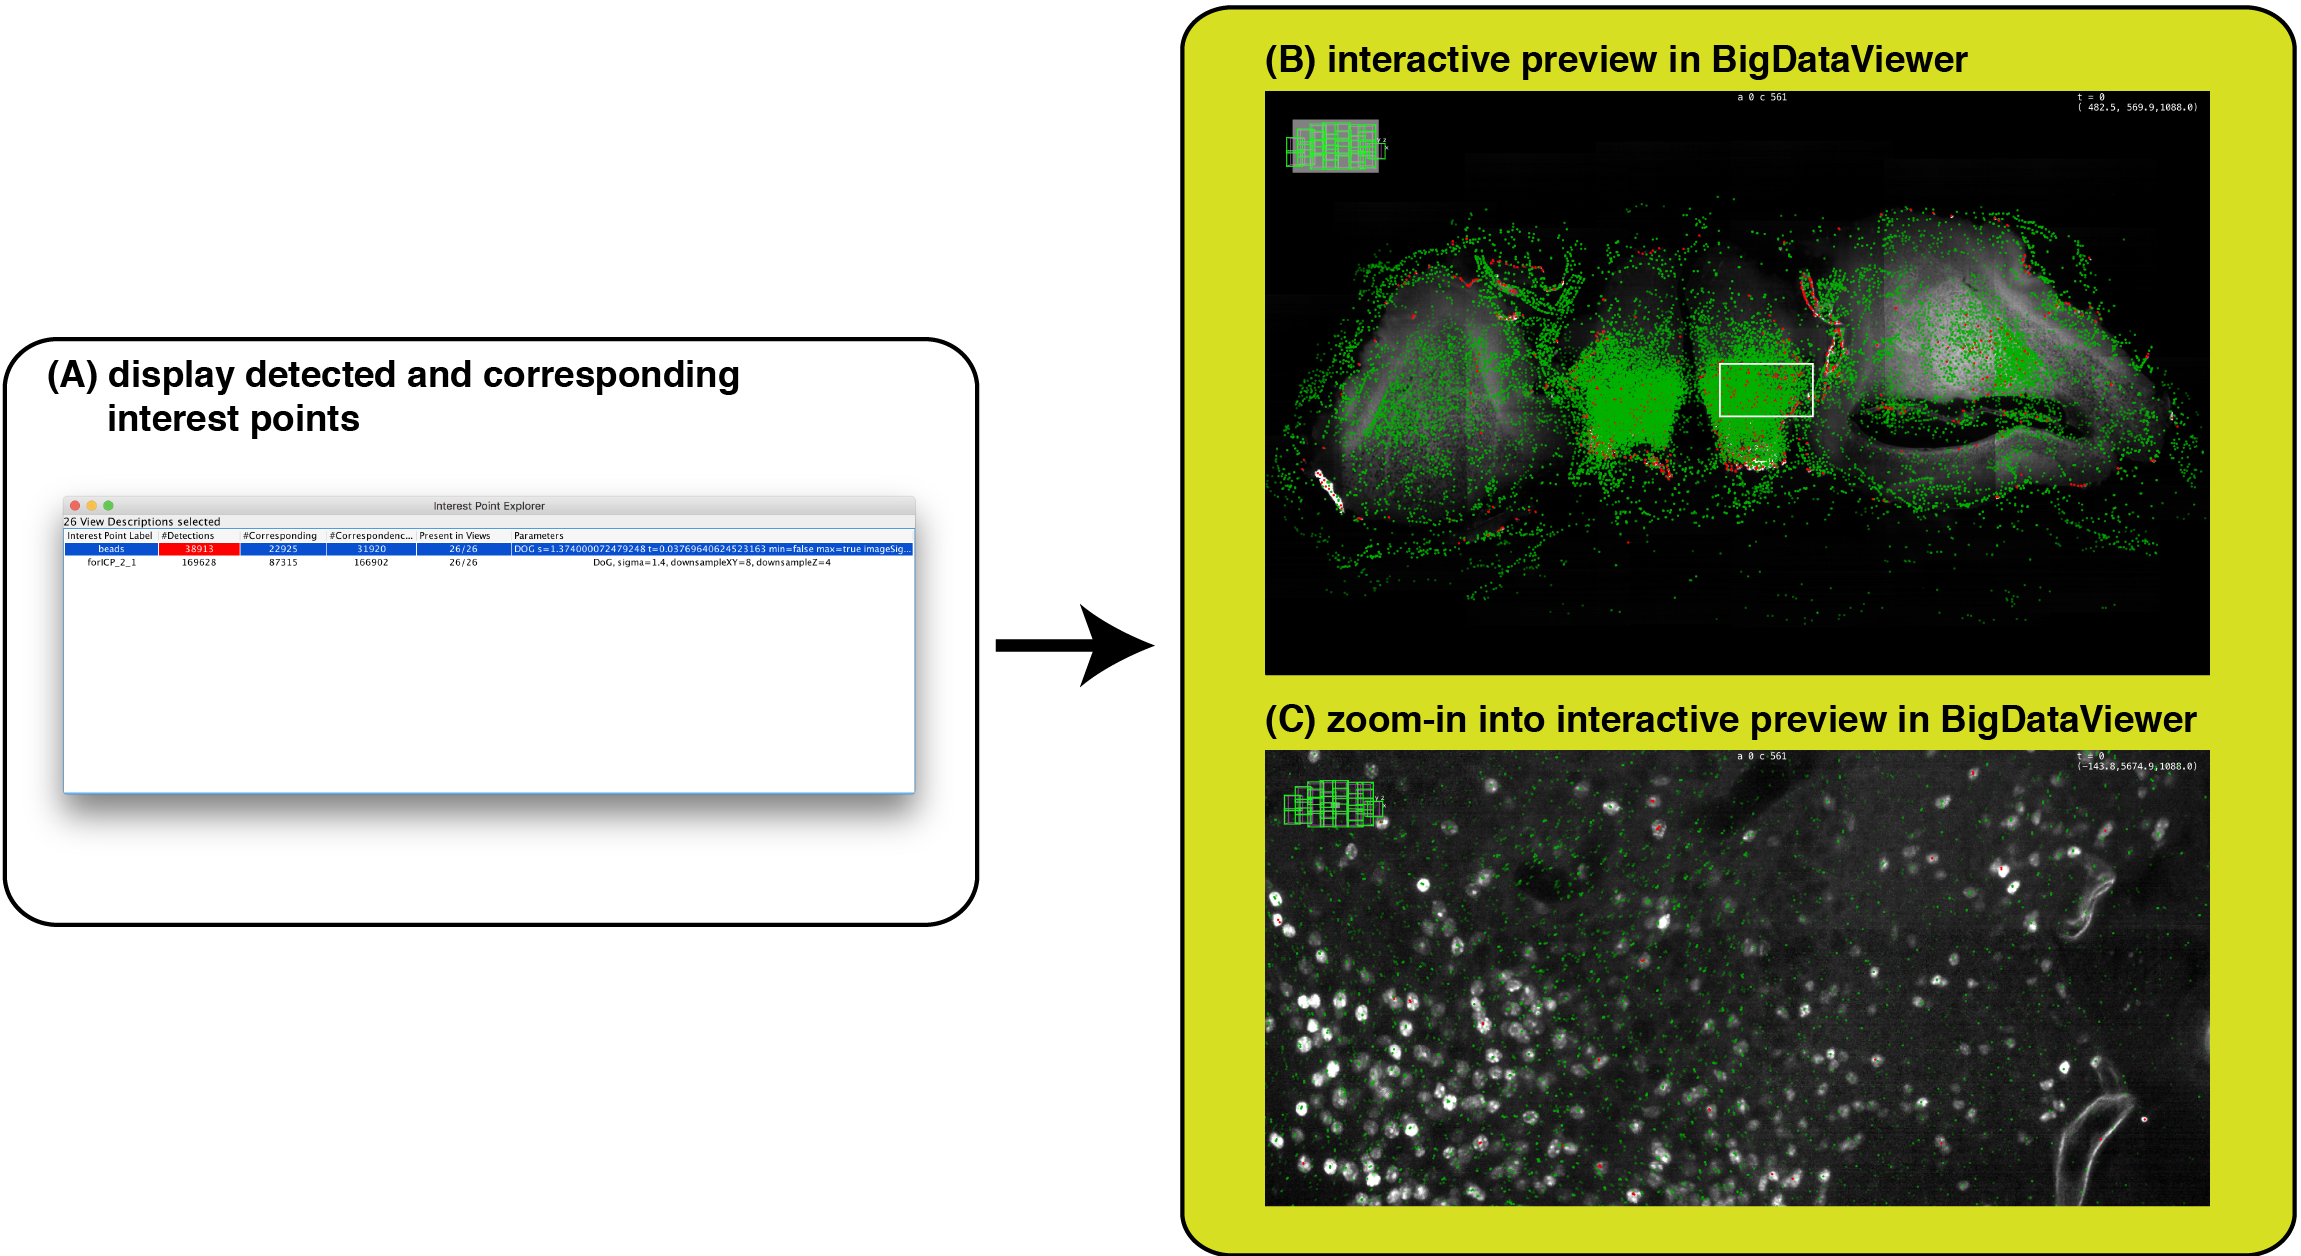
\includegraphics[width=\textwidth]{Supp-IntrestPoints.png}
\vspace{-2.0mm}
\caption{\hspace{-0.5mm} \emph{Interactive visualization of interest points.} The interest points explorer allows the visualization of interest points and corresponding interest points between views. \textbf{(A)} select desired interest points for visualization. \textbf{(B)} preview the interest points overlaid in the BigDataViewer.
}
\label{fig:sup-fig-interest-point}
\end{figure*}

\pagebreak


\subsection*{SUPPLEMENTARY FIGURE 16: Manual Transformation of multi-view datasets}
\vspace{1mm}
\begin{figure*}[h!]
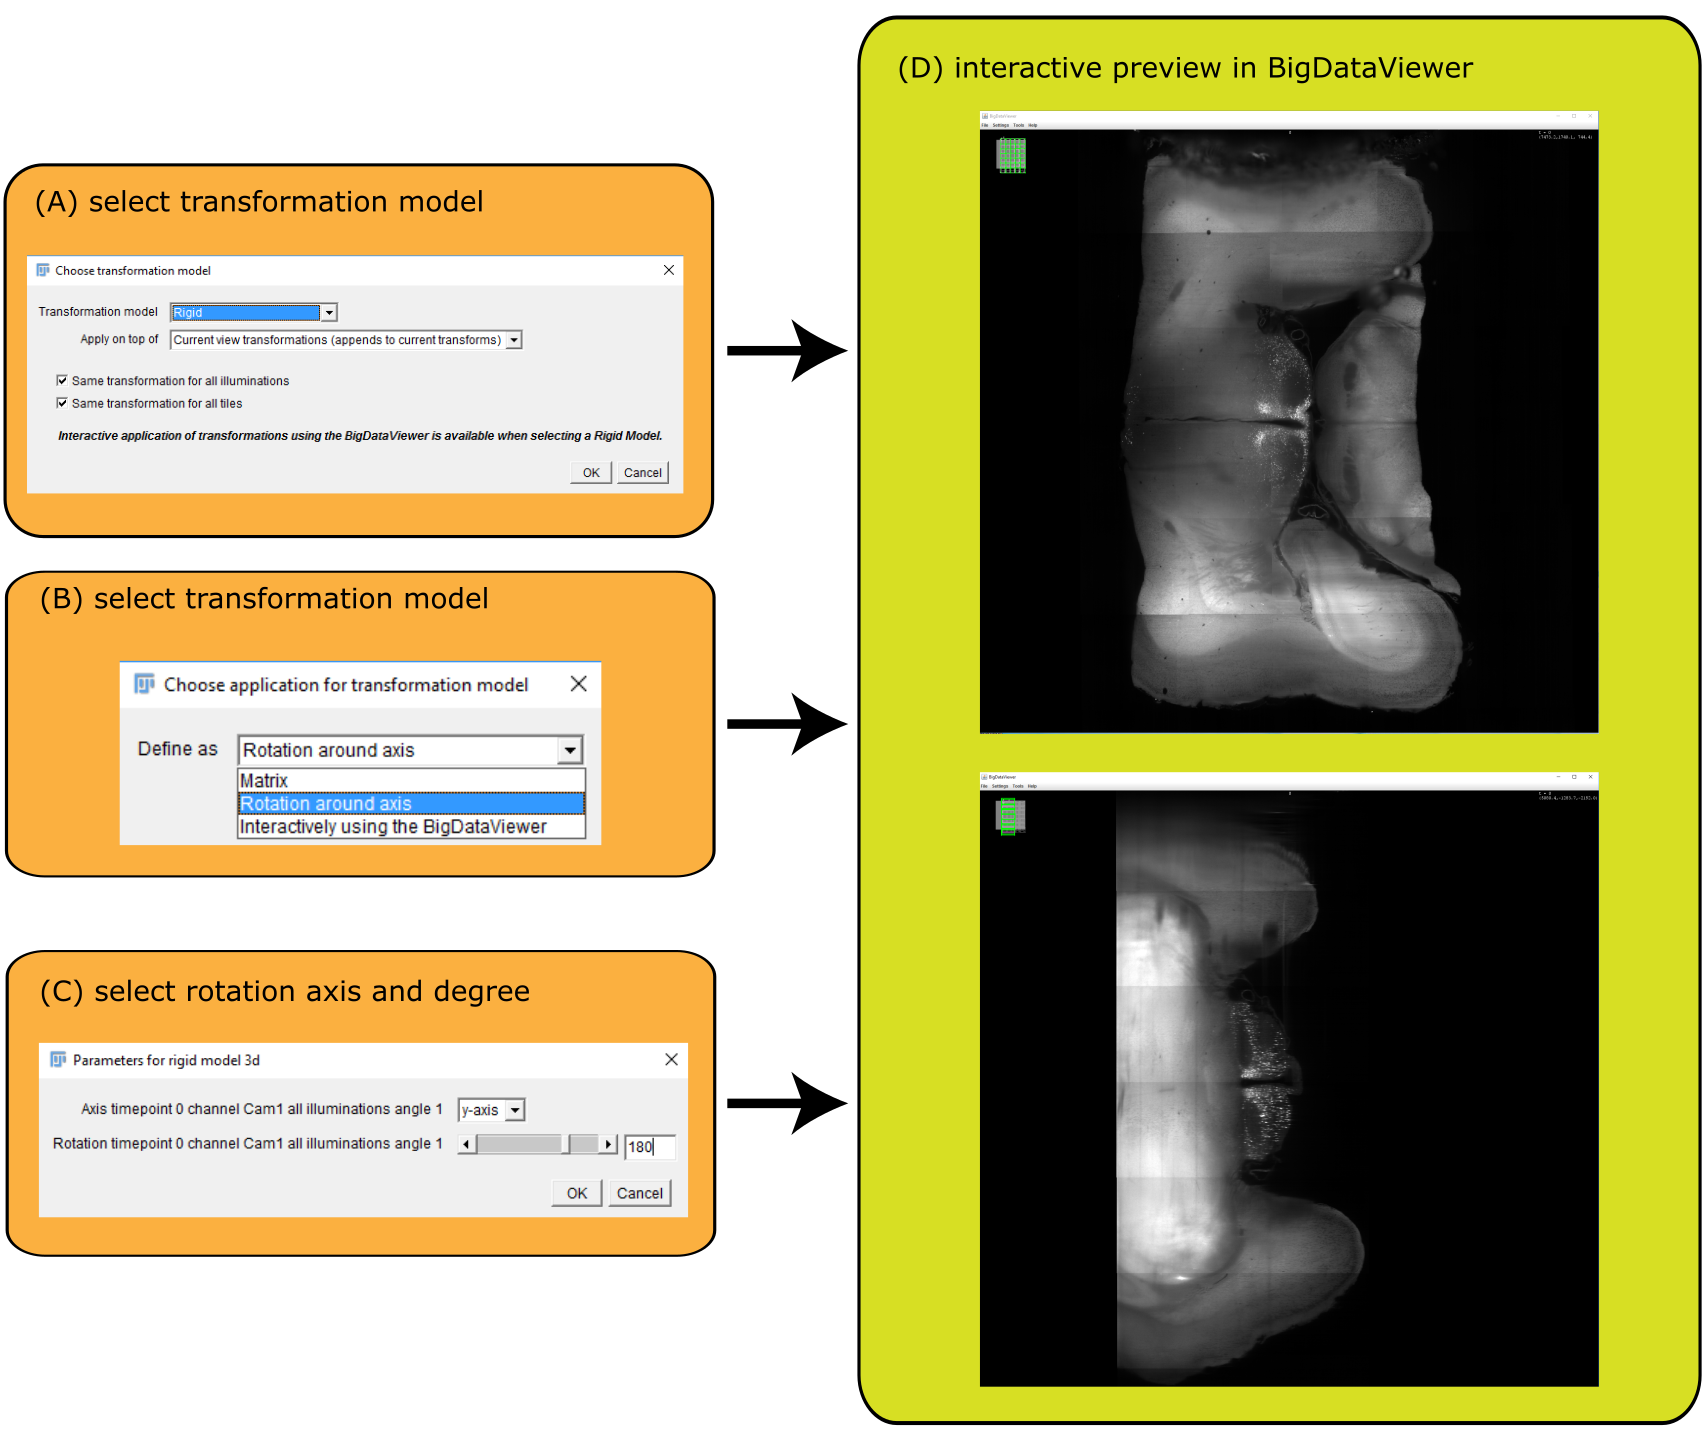
\includegraphics[width=\textwidth]{Supp-Transformation.png}
\vspace{-2.0mm}
\caption{\hspace{-0.5mm} \emph{Interactive transformation of views.} Different transformation models can be applied to one or more views and simultaneously visualized in the BigDataViewer. \textbf{(A)} Choose transformation model grouping. \textbf{(B)} Further define the transformation model. In this case a rotation around the axis is selected. \textbf{(C)} Select rotation axis and angle. \textbf{(D)} Visualize rotation of the view in the BigDataViewer.
}
\label{fig:sup-fig-manual-align2}
\end{figure*}

\pagebreak

\subsection*{SUPPLEMENTARY FIGURE 17: Expansion Microscopy Stitching}
\vspace{1mm}
\begin{figure*}[h!]
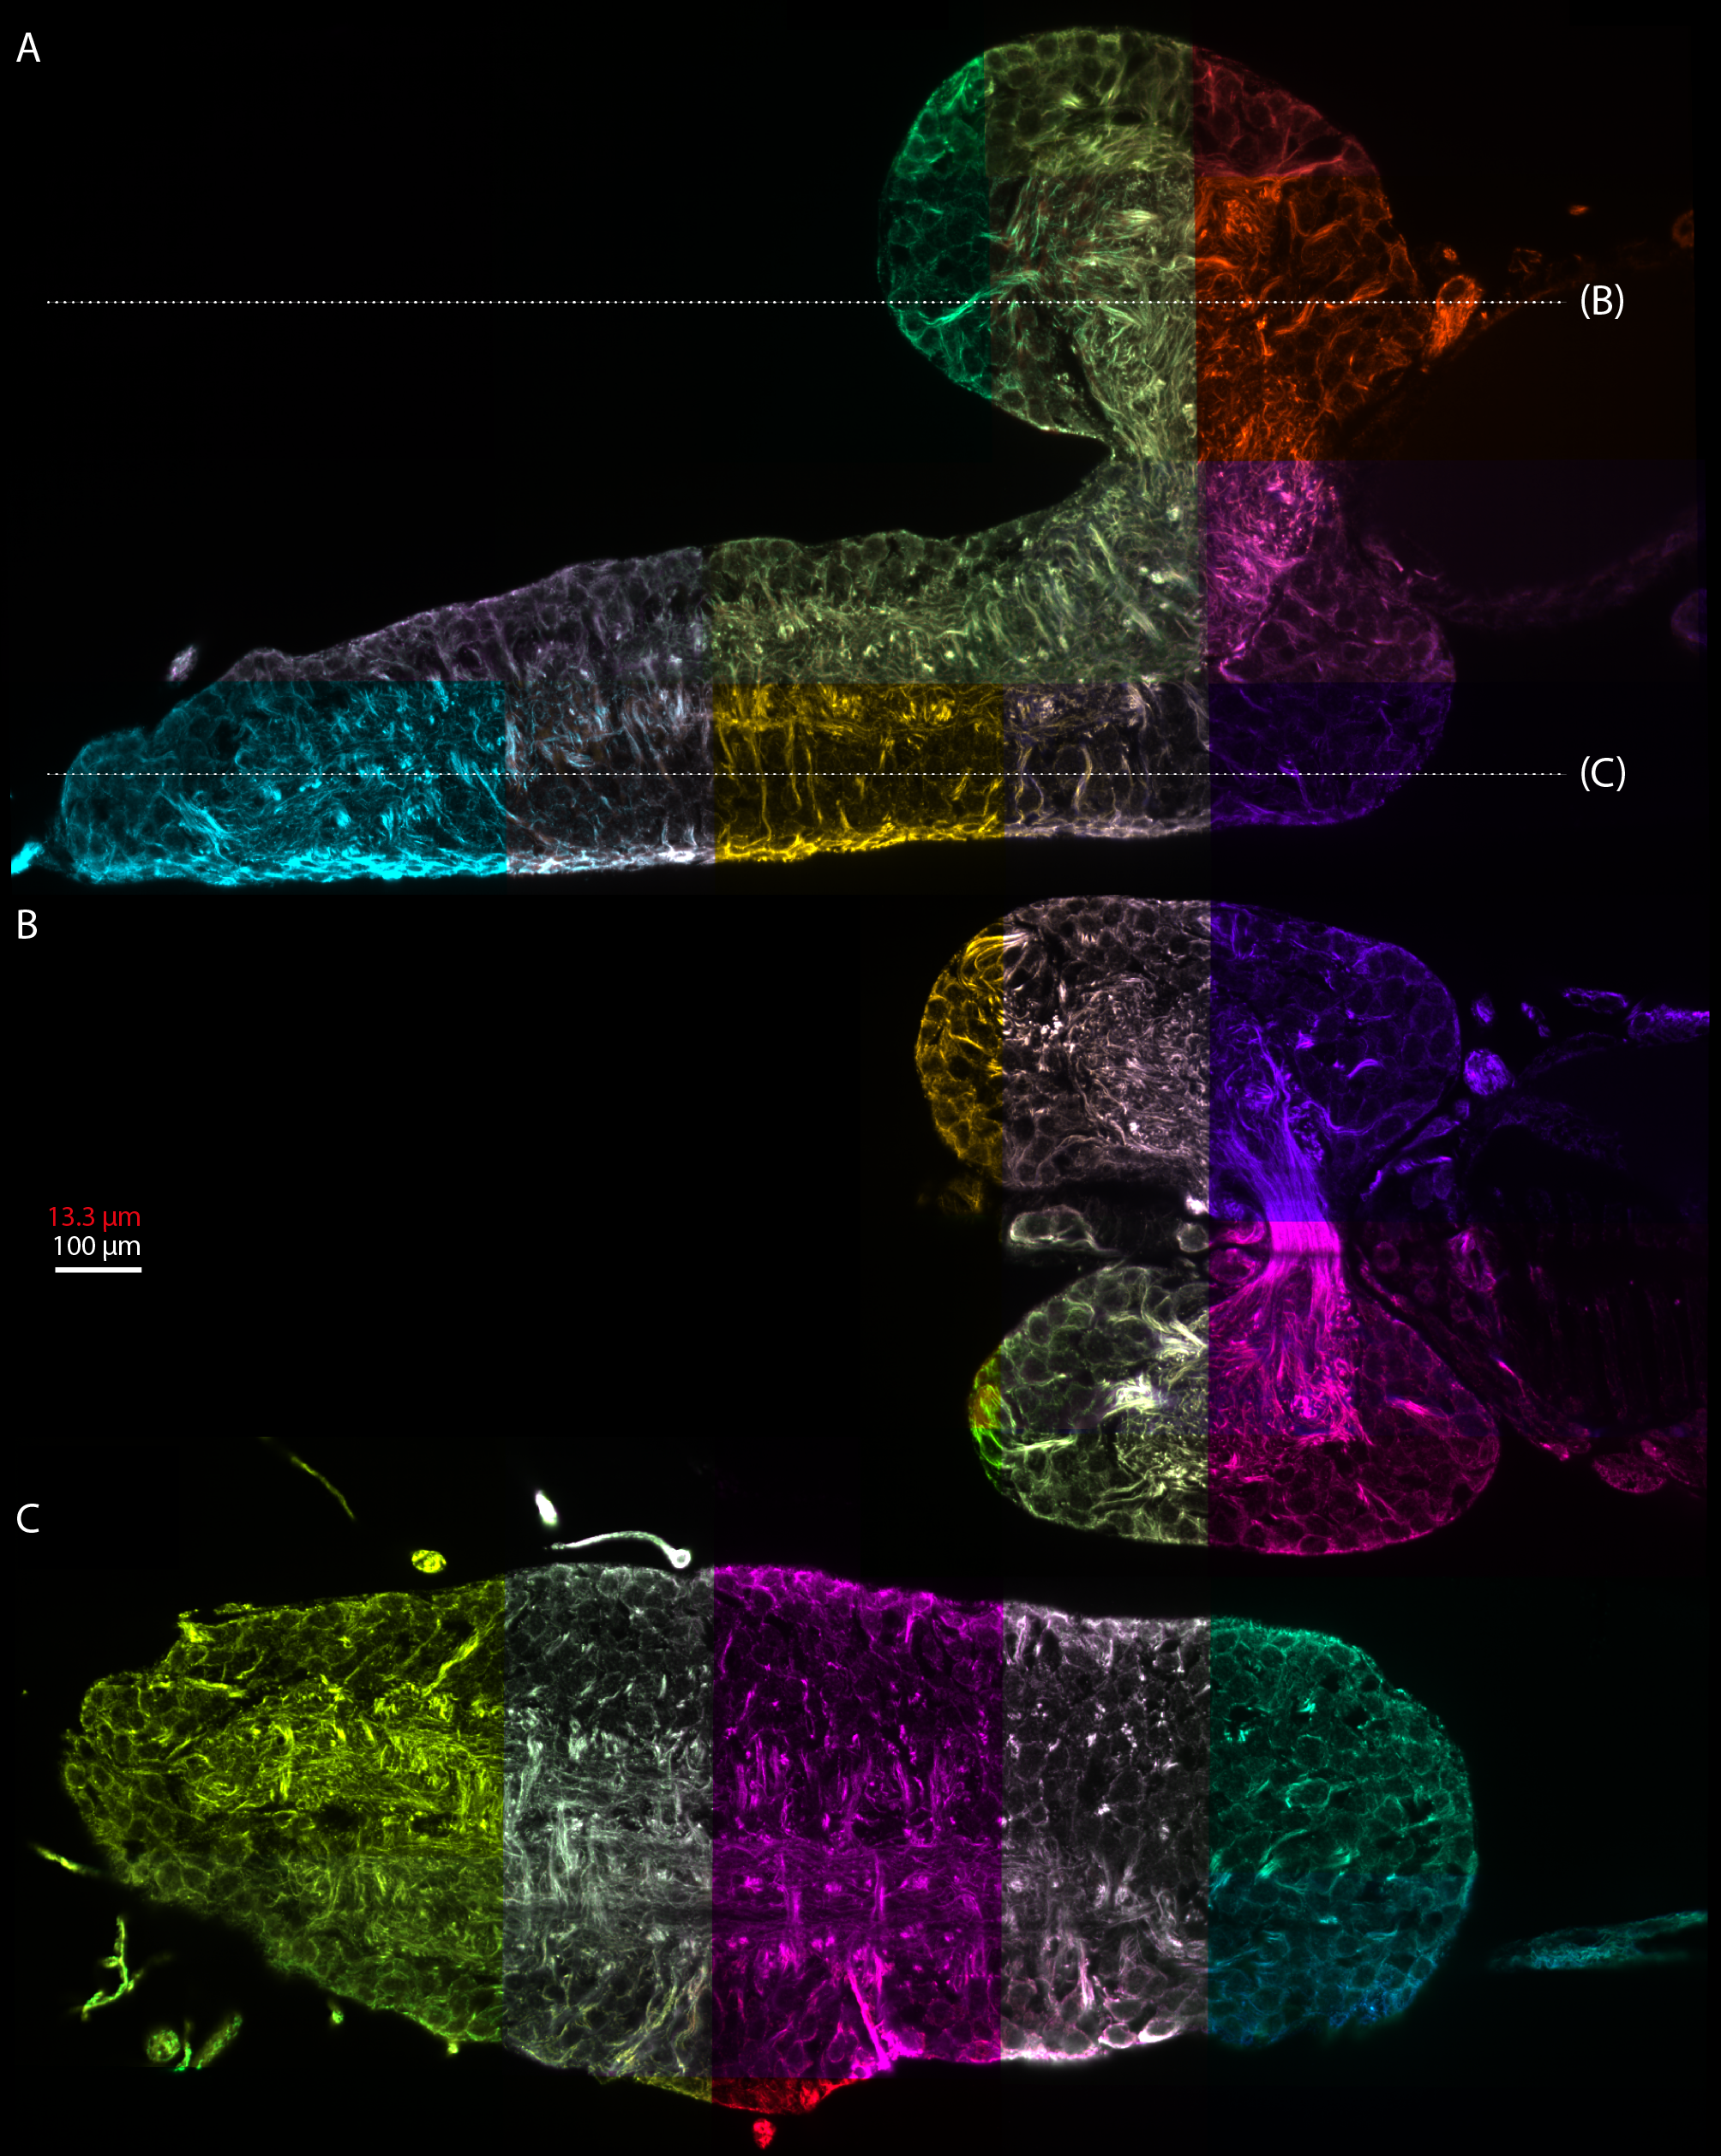
\includegraphics[width=\textwidth]{fig-expansion_tiling.png}
\vspace{-2.0mm}
\caption{\hspace{-0.5mm} \emph{Stitching of a single view of the expansion microscopy sample} All stitched tiles of one view of the expanded Drosophila central nervous system. Each tile is randomly colored to illustrate the overlap regions in between the stacks.
}
\label{fig:sup-fig-expansion-microscopy}
\end{figure*}

\pagebreak

\input supplementary-methods.tex

%\titleformat{\section}{\centering\normalfont\fontsize{13.5pt}{1em}\bfseries}{SUPPLEMENTARY NOTE \thesection: }{0em}{}
\section{BigStitcher User Guide}
\label{sec:documentation}

\subsection{This is where the documentation will go}

Lorem ipsum dolor sit amet.

\pagebreak

% description of current version location is in currentcode.tex 
\input currentcode.tex


%\section{OTHER RELATED LITERATURE}
%The field of multi-view deconvolution is large and diverse; many areas of science contribute including medical science, astronomy, microscopy and the classical computer science. Within the focus of this publications it is not possible to discuss all aspects (e.g. multi-channel deconvolution). We therefore list other publications that contributed to various aspects of multi-image deconvolution\cite{Rajagopalan1998, Giannakis2000, Flusser2003, Vieilleville2011, heintzmann2002, ShawAl89,agard1984,agard1989,verveer1998,heintzmann2000,holmes1991,blume2007}.


%%%%%%%%%%%%%%%%%%%%%%%%%%%%%%%%%%%%%%%%%%%%%%%%%%%%%%%%%%%%%
%\acknowledgments     %>>>> equivalent to \section*{ACKNOWLEDGMENTS}

%%%%%%%%%%%%%%%%%%%%%%%%%%%%%%%%%%%%%%%%%%%%%%%%%%%%%%%%%%%%%
%%%%% References %%%%%

\bibliography{supplement-bibliography}   %>>>> bibliography data in supplement-bibliography.bib
\bibliographystyle{spiebib}   %>>>> makes bibtex use spiebib.bst

\end{document}
